\documentclass[12pt,oneside]{report}
\usepackage[letterpaper,margin=1in]{geometry}
\usepackage{fontspec}
\setmainfont{Times New Roman}
\usepackage{setspace}
\onehalfspacing
\usepackage{graphicx}
\usepackage{longtable,booktabs,array,tabularx}
\newcolumntype{W}{>{\raggedright\arraybackslash}X}
\newcolumntype{P}[1]{>{\raggedright\arraybackslash}p{#1}}
\newcolumntype{C}{>{\raggedright\arraybackslash}p{0.24\textwidth}}
\setlength{\tabcolsep}{3pt}
\usepackage{amsmath,amssymb}
\usepackage[hidelinks]{hyperref}
\usepackage{xurl}
\usepackage{tikz}
\usetikzlibrary{arrows.meta, positioning}
\usepackage{fancyhdr}
\setlength{\parindent}{0pt}
\setlength{\parskip}{6pt}
\begin{document}
\section*{Shor's Algorithm and Post-Quantum Payment Cryptography}
\addcontentsline{toc}{section}{Shor's Algorithm and Post-Quantum Payment Cryptography}

\begin{center}
\textbf{Mathematical foundations of Shor’s algorithm and its implications for post-quantum payment cryptography}
\par

\textbf{Dissertation Report}
\par

Submitted in partial fulfilment of the requirements for the
\par

\textbf{A}\textbf{ward of the degree of}
\par

"Master of Science (Mathematics)"
\par

\textbf{Submitted By}: Parag P Kulkarni
\par
\textbf{Registration No}: 324200584
\par

\textbf{Supervisor}: Dr. Prerna, Assistant Professor (Senior), Mathematics Department, LPU
\par
\textbf{UID}: 33588
\par

\begin{center}
\includegraphics[width=0.82\textwidth]{assets/image1.png}\end{center}
\par

\textbf{Centre for Distance and Online Education}
\par

\textbf{LOVELY PROFESSIONAL UNIVERSITY, }
\par

\textbf{PHAGWARA, PUNJAB }
\par

\textbf{2026}
\end{center}
\par
\newpage

Student Declaration (Annexure III)
\par

To Whom-so-ever it may concern
\par

I, \textbf{Parag P Kulkarni, [324200584]}, hereby declare that the work done by me on "\textbf{Mathematical Foundations of Shor's Algorithm and Its Implications for Post-Quantum Payment Cryptography}" under the supervision of Dr. Prerna, Assistant Professor, Lovely Professional University, Phagwara, Punjab, is a record of original work for the partial fulfilment of the requirements for the award of the degree, \textbf{Master of Science (Mathematics)}. As for the contributions of others are concerned, all efforts have been made to indicate clearly. The \textbf{dissertation} is also checked by plagiarism software. If there will be any issue regarding originality and plagiarism, the undersigned will be responsible, and the awarded degree may be cancelled.
\par

\textbf{Name of the Student}: Parag P Kulkarni [324200584]
\par

Signature of the Student:
\par

\begin{flushleft}
\includegraphics[width=2.2cm,height=1.5cm,keepaspectratio]{assets/image2.jpeg}\end{flushleft}
\par

Dated: 19-Nov-2026
\par

\newpage
\subsection*{Certificate by the Supervisor (Annexure IV)}
\addcontentsline{toc}{subsection}{Certificate by the Supervisor (Annexure IV)}

To Whom-so-ever it may concern
\par

This is to certify that \textbf{Parag P Kulkarni, [324200584]}, from Lovely Professional University, Phagwara, Punjab, has worked on "\textbf{Mathematical Foundations of Shor's Algorithm and Its Implications for Post-Quantum Payment Cryptography}" under my supervision. It is further stated that the work carried out by the student is a record of original work to the best of my knowledge for the partial fulfilment of the requirements for the award of the degree, Master of Science (Mathematics). The originality of the research work is also verified by well-developed plagiarism software.
\par

Name of Supervisor:Dr. Prerna, Assistant Professor (Senior), Mathematics Department, LPU
\par

UID of Supervisor: 33588
\par

Signature of Supervisor:
\par

\subsection*{Acknowledgement}
\addcontentsline{toc}{subsection}{Acknowledgement}

I want to thank the Lovely Professional University and my professors, including Dr. Isha Garg and Dr. Prerna, for providing me with this opportunity to work on the topic of my personal interest, as part of my final semester dissertation.
\par

\newpage
\subsection*{Table of Contents}
\addcontentsline{toc}{subsection}{Table of Contents}

\begin{center}\small\begin{tabularx}{\textwidth}{|W|W|W|}\hline
S. No. & Title & Page \\\hline
1 & Declaration by Student & 2 \\\hline
2 & Certificate by Supervisor & 3 \\\hline
3 & Acknowledgement & 3 \\\hline
4 & List of Tables & 5 \\\hline
5 & List of Figures / Charts & 6 \\\hline
6 & List of Abbreviations & 7 \\\hline
7 & Chapter 1 Introduction & 9 \\\hline
8 & Chapter 2 Review of Literature & 14 \\\hline
9 & Chapter 3 Work Plan & 20 \\\hline
10 & Chapter 4 Results and Discussions & 28 \\\hline
11 & Chapter 5 Conclusion and Future Perspectives & 45 \\\hline
12 & Chapter 6 List of Publications / Conference Papers & 48 \\\hline
13 & References & 48 \\\hline
14 & Plagiarism Report & 53 \\\hline
\end{tabularx}\end{center}

\subsection*{List of Tables}
\addcontentsline{toc}{subsection}{List of Tables}

\begin{center}\small\begin{tabularx}{\textwidth}{|P{0.1\textwidth}|W|P{0.1\textwidth}|}\hline
Table & Title & Page \\\hline
2.1 & Summary of reviewed literature by theme & \pageref{tab:2.1} \\\hline
2.2 & Published resource estimates for breaking RSA-2048 and ECC-256 & \pageref{tab:2.2} \\\hline
3.1 & Operational definitions of study variables & \pageref{tab:3.1} \\\hline
3.2 & Integers and bases selected for simulation & \pageref{tab:3.2} \\\hline
3.3 & Payment components and estimated time parameters & \pageref{tab:3.3} \\\hline
3.4 & Analysis techniques by objective & \pageref{tab:3.4} \\\hline
4.1 & Observed versus theoretical success of period finding & \pageref{tab:4.1} \\\hline
4.2 & Success funnel for all 22 cases & \pageref{tab:4.2} \\\hline
4.3 & Period recovered against counting qubits & \pageref{tab:4.3} \\\hline
4.4 & Independent verification with SymPy & \pageref{tab:4.4} \\\hline
4.5 & Circuit resources after compilation ($a = 2$) & \pageref{tab:4.5} \\\hline
4.6 & Success rate under increasing gate error ($N = 15$, $a = 7$, 4,096 runs each) & \pageref{tab:4.6} \\\hline
4.7 & IBM Quantum hardware runs & \pageref{tab:4.7} \\\hline
4.8 & Hardware results for $N = 15$, $a = 7$ (runs A and B) & \pageref{tab:4.8} \\\hline
4.9 & Hardware results for period 6 ($N = 21$, $a = 2$ and $N = 77$, $a = 12$; runs C, D and E) & \pageref{tab:4.9} \\\hline
4.10 & Grover key-search cost for AES ($\log_{2}$ of Grover iterations) & \pageref{tab:4.10} \\\hline
4.11 & Quantum exposure of payment-system components & \pageref{tab:4.11} \\\hline
4.12 & Migration priority scores and ranking & \pageref{tab:4.12} \\\hline
4.13 & Monte Carlo sensitivity analysis & \pageref{tab:4.13} \\\hline
4.14 & Summary of hypothesis test results & \pageref{tab:4.14} \\\hline
\end{tabularx}\end{center}

\subsection*{List of Figures / Charts}
\addcontentsline{toc}{subsection}{List of Figures / Charts}

\begin{center}\small\begin{tabularx}{\textwidth}{|P{0.1\textwidth}|W|P{0.1\textwidth}|}\hline
Figure & Title & Page \\\hline
1.1 & Structure of the dissertation & \pageref{fig:1.1} \\\hline
4.1 & Quantum circuit for period finding ($N = 15$, $a = 7$) & \pageref{fig:4.1} \\\hline
4.2 & Simulated and theoretical outcome distributions for $N = 15$, $a = 7$ (period 4) & \pageref{fig:4.2} \\\hline
4.3 & Simulated and theoretical outcome distributions for $N = 21$, $a = 2$ (period 6) & \pageref{fig:4.3} \\\hline
4.4 & Observed and theoretical success per run for all 13 cases & \pageref{fig:4.4} \\\hline
4.5 & Success funnel for selected cases: useful phase estimate, period recovered and factor recovered & \pageref{fig:4.5} \\\hline
4.6 & Period recovery against the number of counting qubits & \pageref{fig:4.6} \\\hline
4.7 & Two-qubit gate count and circuit depth against the bit-length of N & \pageref{fig:4.7} \\\hline
4.8 & Success rate against two-qubit gate error rate, with the noise-free value and the 8.6\% rate expected from random outcomes & \pageref{fig:4.8} \\\hline
4.9 & Measured distributions for $N = 15$, $a = 7$ on ibm\_fez and ibm\_marrakesh, compared with theory & \pageref{fig:4.9} \\\hline
4.10 & Measured distributions for the period-6 circuit & \pageref{fig:4.10} \\\hline
4.11 & Shelf life plus migration time for each component (dot = most likely value, bar = low-to-high range) against the near, central and late threat scenarios & \pageref{fig:4.11} \\\hline
\end{tabularx}\end{center}

\subsection*{List of Abbreviations}
\addcontentsline{toc}{subsection}{List of Abbreviations}

\begin{center}\small\begin{tabularx}{\textwidth}{|W|W|}\hline
Abbreviation & Full Form \\\hline
3DES & Triple Data Encryption Standard \\\hline
AES & Advanced Encryption Standard \\\hline
ARQC & Authorisation Request Cryptogram \\\hline
CDA & Combined Data Authentication \\\hline
CRQC & Cryptographically Relevant Quantum Computer \\\hline
CRT & Chinese Remainder Theorem \\\hline
CZ & Controlled-Z (two-qubit gate) \\\hline
DD & Dynamical Decoupling \\\hline
DDA & Dynamic Data Authentication \\\hline
ECC & Elliptic-Curve Cryptography \\\hline
ECDLP & Elliptic-Curve Discrete Logarithm Problem \\\hline
EMV & Europay, Mastercard and Visa (chip card standard) \\\hline
FIPS & Federal Information Processing Standard \\\hline
HSM & Hardware Security Module \\\hline
ML-DSA & Module-Lattice-Based Digital Signature Algorithm \\\hline
ML-KEM & Module-Lattice-Based Key-Encapsulation Mechanism \\\hline
NIST & National Institute of Standards and Technology \\\hline
NISQ & Noisy Intermediate-Scale Quantum \\\hline
PQC & Post-Quantum Cryptography \\\hline
QFT & Quantum Fourier Transform \\\hline
RSA & Rivest–Shamir–Adleman \\\hline
SDA & Static Data Authentication \\\hline
TLS & Transport Layer Security \\\hline
TVD & Total Variation Distance \\\hline
UPI & Unified Payments Interface \\\hline\end{tabularx}\end{center}

\newpage
\section*{Dissertation Summary}
\addcontentsline{toc}{section}{Dissertation Summary}

Registration No: 324200584
\par

Name of Student: Parag P Kulkarni
\par

Title of the Dissertation: Mathematical Foundations of Shor's Algorithm and Its Implications for Post-Quantum Payment Cryptography
\par

Objectives of the Dissertation:

\begin{itemize}

\item To present the mathematical foundations of quantum period finding and Shor's algorithm using concepts from group theory, number theory and Fourier analysis.
\par

\item To simulate Shor's algorithm for small composite integers and compare observed success probabilities with theoretical values.
\par

\item To distinguish the impact of Shor's and Grover's algorithms on the cryptographic mechanisms used in payment systems.
\par

\item To rank payment-system components by quantum migration priority using a scoring method based on Mosca's inequality.
\end{itemize}
\par

\textbf{Results and Findings:} Simulated success rates of Shor's algorithm matched theory in all 22 cases from $N = 15$ to $N = 55$ (combined $p = 0.692$), and every failure matched a theoretically predicted cause. Period recovery depended on phase-estimation precision exactly as continued-fraction theory predicts. Under a depolarising noise model, a 1\% two-qubit error rate reduced success from 50.3\% to 28.7\%. On IBM quantum hardware, the factors 3 and 5 of N = 15 were recovered in 45.8\% and 40.6\% of shots on two devices (ideal 50\%); a period-6 experiment for N = 21 and N = 77 recovered a statistically significant signal on two devices after the circuit was redesigned using the Chinese Remainder Theorem and the semi-classical Fourier transform. Grover's algorithm only reduces the security margin of AES: under a realistic depth limit, AES-128 requires about $2^{87}$ iterations and AES-256 retains a substantial margin under the assumptions considered. Under the study's scoring assumptions, HSM key transport, EMV offline data authentication and TLS key exchange are the top three migration priorities; certificates, though broken by Shor's algorithm, rank last because of their short lifetimes.
\par

\textbf{Specific Outcomes of the Dissertation:} A reproducible Qiskit simulation of Shor's algorithm with statistical validation; a component-level quantum exposure map for payment systems distinguishing Shor and Grover effects; a reusable migration-priority scoring framework with sensitivity analysis; and five executions on IBM quantum hardware comparing three devices and two circuit designs. 
\par

Learnings from the Dissertation:
When I started with this topic, I was just curious about the quantum computing part of it. But I was not aware of the true connection between the cryptographic algorithms like RSA, Elliptic Curve Cryptography (ECC) and the quantum computers in the sense that how Shor's and Grover's algorithms can enable them to break. I found out that the quantum part of the Shor's algorithm actually solves the hard problem that the classical computers cannot solve in polynomial time - finding the period (or order) r of a modular function by using quantum superposition and the Quantum Fourier Transform (QFT) to compute all possible values at once. The algorithm prepares a quantum register in a uniform superposition of numbers using Hadamard gates. This allows the quantum computer to evaluate the modular exponentiation function for all those numbers simultaneously. 

        \[ f(x) = a^x \pmod{N} \]

        Now a second register stores the result of the above computation. I learned that because the function is periodic, the entire state becomes entangled into repeating wave-like pattern where the period is r.

This was the moment I started worrying about how to practically show this without an actual quantum computer. But I had learned about IBM's and Google's quantum computers so I searched online for ways to use those. That's when I found the Qiskit toolkit, that can actually be used to program these Hadamard gates and submit a job to a cloud based quantum computer or even a simulator to perform these actions. Of course the semiprime numbers I could choose were extremely small - like 15 and 21. 

\par

Any Challenges / Issues Faced during the Dissertation:
\par

Signature of the Student:
\par

\begin{flushleft}
\includegraphics[height=16pt,keepaspectratio]{assets/image2.jpeg}\end{flushleft}
\par

\newpage
\section*{Chapter 1: Introduction}
\addcontentsline{toc}{section}{Chapter 1: Introduction}

\subsection*{1.1 Background}
\addcontentsline{toc}{subsection}{1.1 Background}

The security of modern digital payments rests on a small number of mathematical problems believed to be hard for classical computers. Public-key cryptosystems such as RSA (Rivest et al., 1978) depend on the difficulty of factoring large integers. Elliptic-curve cryptography (Koblitz, 1987; Miller, 1986) depends on the difficulty of the elliptic-curve discrete logarithm problem. These systems authenticate chip cards, protect key exchange in TLS sessions, sign transactions and wrap cryptographic keys inside hardware security modules.
\par

In 1994, Peter Shor showed that a quantum computer could solve both problems in polynomial time (Shor, 1994, 1997). The algorithm converts factoring into a problem of finding the period of a modular function. That period is extracted efficiently using the Quantum Fourier Transform, a quantum analogue of the discrete Fourier transform. A second, more limited result followed from Grover (1996), discussed below.
\par

For many years, these results were of theoretical interest only, because building a large, error-corrected quantum computer appeared distant. That view has since changed. Resource estimates for breaking RSA have fallen sharply, and standards bodies have responded: in 2024 the U.S. National Institute of Standards and Technology (NIST) published its first post-quantum cryptography standards (NIST, 2024a, 2024b, 2024c).
\par

Grover (1996) showed a second, weaker effect. Quantum search finds a hidden key among N possibilities in about $\sqrt{N}$ steps instead of N. For symmetric ciphers such as AES, this reduces the security margin — the gap between the effort needed to break the cipher and the effort any attacker can realistically spend — but does not eliminate it, and longer keys restore it (Bernstein \& Lange, 2017; Chen et al., 2016). Public-key systems and symmetric systems are therefore threatened in fundamentally different ways.
\par

The threat has moved from theory towards planning. Estimates of the resources needed to factor RSA-2048 have fallen from about 20 million noisy qubits under the assumptions of Gidney and Ekerå (2021) to fewer than one million under the different assumptions in Gidney (2025). These are conditional resource estimates, not evidence that a cryptographically relevant quantum computer is currently available. Google Quantum AI and collaborators (2025) demonstrated below-threshold surface-code error correction, an important milestone but not a demonstration of Shor’s algorithm at cryptographic scale. In 2024, the U.S. National Institute of Standards and Technology (NIST) published the first post-quantum cryptography standards, ML-KEM and ML-DSA (NIST, 2024a, 2024b).
\par

Payments require advance planning because cryptographic dependencies, terminals, cards, hardware security modules and supporting infrastructure can have long service and replacement cycles. Recorded encrypted traffic may be vulnerable to “harvest now, decrypt later” (Joseph et al., 2022; Mosca, 2018) attacks where long-term confidentiality is required. This concern is distinct from the threat to public-key authentication and key establishment, and its relevance depends on the data and protocol involved (Mosca, 2018). Organisations therefore need to inventory cryptographic dependencies and prioritise migration.
\par

The principal concern is not that quantum computers will compromise all card payments simultaneously. The risk is concentrated in public-key cryptography used for offline authentication, with additional migration considerations for remote payments and the wider payments infrastructure.
\par

Payment networks, issuers, acquirers and technology providers should monitor cryptographic dependencies, assess where RSA and ECC are used, and plan for eventual migration to post-quantum cryptography (PQC). There is no immediate requirement to replace all EMV chip technology solely because of quantum computing. However, EMVCo states that it does not expect quantum computing to pose a threat to EMV infrastructure until at least 2040, while acknowledging that no one knows when such a threat will arrive (EMVCo, 2025). Online EMV cryptograms, by contrast, use symmetric cryptography, either AES or legacy Triple DES. AES offers strong resistance to known quantum attacks, while Triple DES has a smaller security margin.
\par

This study examines the mathematical foundations of Shor's algorithm, validates them through simulation, and applies the resulting understanding to rank payment-system components by quantum migration priority.
\par

Variables of the study. The study works with the following variables, defined formally in section 3.5. For simulation, “success” means that a run yields a candidate period which, after classical post-processing and verification, produces a non-trivial factor; period-estimation success and factor-recovery success will be reported separately wherever useful.
\par

\textbf{Success probability} of simulated period finding, observed and theoretical.
\par

Quantum exposure class of each cryptographic mechanism: broken (by Shor's algorithm), weakened (by Grover's algorithm) or resistant.
\par

Security shelf life (x), migration time (y) and quantum threat horizon (z) for each payment component, the three terms of Mosca's (2018) risk inequality.
\par

Migration priority score, derived from the three terms above and the exposure class.
\par

\subsection*{1.2 Aim of the Study}
\addcontentsline{toc}{subsection}{1.2 Aim of the Study}

The aim of this study is to examine the mathematical foundations of Shor's algorithm and to assess, in a structured and quantitative way, its implications for cryptography used in payment systems. The study connects the algebra and number theory behind quantum period finding to a practical question: which components of payment infrastructure must migrate to post-quantum cryptography first.
\par

\subsection*{1.3 Importance of the Study}
\addcontentsline{toc}{subsection}{1.3 Importance of the Study}

The study is important for three reasons. First, the quantum threat to public-key cryptography is no longer speculative; published resource estimates and hardware progress indicate a credible timeline for migration planning (Joseph et al., 2022). Second, the threat is uneven. Shor's algorithm breaks RSA and ECC completely, while Grover's algorithm only reduces the security margin of symmetric cryptography. Payment systems use both, so a precise distinction is needed to avoid both complacency and over-reaction. Third, migration in financial infrastructure takes many years, which means priorities must be set well before a quantum computer capable of breaking current cryptography is built (Mosca, 2018).
\par

\subsection*{1.4 Scope of the Study}
\addcontentsline{toc}{subsection}{1.4 Scope of the Study}

In line with section 1.3 of the LPU Dissertation Guidelines, the study addresses the following scope areas:
\par

\begin{itemize}
  \sloppy
  \item Industrial issues (1.3 b): the vulnerability of cryptography embedded in card networks, payment gateways and bank infrastructure.
  \item Government and policy issues (1.3 c): alignment with national and international post-quantum migration efforts, including NIST's standards and India's National Quantum Mission (Press Information Bureau, 2023).
  \item Business issues (1.3 d): prioritising migration investment across payment-system components.
  \item Enriching discipline knowledge (1.3 g): a structured exposition of the group theory, number theory and Fourier analysis that underpin quantum period finding.
\end{itemize}
\par

The study is limited to the factoring and discrete-logarithm threats posed by Shor's algorithm and the key-search threat posed by Grover's algorithm. Simulation is limited to small composite integers that current quantum simulators can handle. Post-quantum algorithms are assessed as migration targets, not analysed mathematically in depth.
\par

\subsection*{1.5 Applicability and Relevance}
\addcontentsline{toc}{subsection}{1.5 Applicability and Relevance}

The findings are applicable to payment networks, issuing and acquiring banks, payment processors, token service providers and regulators planning cryptographic transitions. The migration-priority framework developed in Chapter 4 can be reused by any organisation to rank its own cryptographic assets. The mathematical exposition is relevant to students and practitioners who need to understand why the quantum threat is real without a background in quantum physics.
\par

In the context of the Indian payment ecosystem, even with UPI, similar challenges exist. It still relies on public-key cryptography such as RSA, ECC for API authentication, digital signatures and merchant QR code verification. So to address such concerns, RBI has constituted a panel from reputed organizations such as NPCI, SBI and IITs to map these cryptographic risks and oversee sector-wise transition. 
\par

\subsection*{1.6 Structure of the Dissertation}
\addcontentsline{toc}{subsection}{1.6 Structure of the Dissertation}

The dissertation is organized into six chapters, as shown in Figure 1.1. Chapter 1 introduces the problem and its scope. Chapter 2 reviews the literature on Shor's and Grover's algorithms, quantum resource estimates, post-quantum standards and cryptographic migration, and identifies research gaps. Chapter 3 sets out the work plan: research problem, objectives, hypotheses, operational definitions, sample, design and analysis techniques. Chapter 4 presents simulation results, the payment-system exposure mapping and the migration-priority ranking. Chapter 5 states conclusions, limitations and future perspectives. Chapter 6 lists publications arising from the work.
\par

\begin{center}
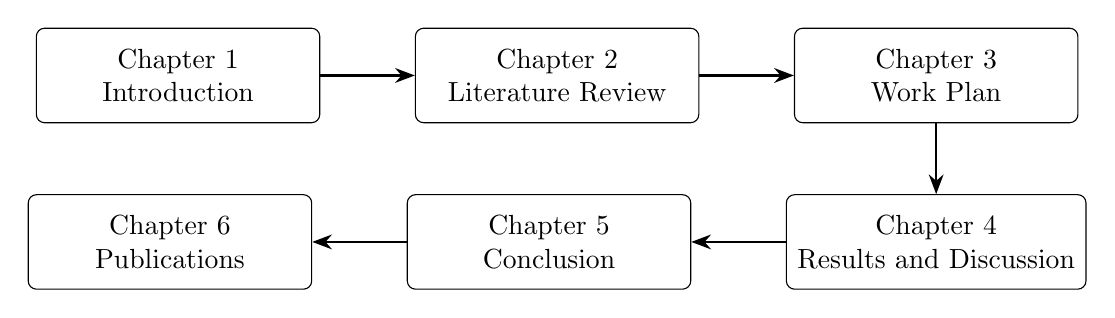
\begin{tikzpicture}[
  box/.style={draw, rounded corners=3pt, align=center, minimum width=3.6cm, minimum height=1.2cm, inner sep=4pt},
  arr/.style={-{Stealth[length=2.5mm]}, thick}]
  \node[box] (c1) {Chapter 1\\Introduction};
  \node[box, right=1.2cm of c1] (c2) {Chapter 2\\Literature Review};
  \node[box, right=1.2cm of c2] (c3) {Chapter 3\\Work Plan};
  \node[box, below=0.9cm of c3] (c4) {Chapter 4\\Results and Discussion};
  \node[box, left=1.2cm of c4] (c5) {Chapter 5\\Conclusion};
  \node[box, left=1.2cm of c5] (c6) {Chapter 6\\Publications};
  \draw[arr] (c1) -- (c2);
  \draw[arr] (c2) -- (c3);
  \draw[arr] (c3) -- (c4);
  \draw[arr] (c4) -- (c5);
  \draw[arr] (c5) -- (c6);
\end{tikzpicture}
\end{center}
\phantomsection\label{fig:1.1}Figure 1.1: Structure of the dissertation
\par

\subsection*{1.7 Chapter Conclusion}
\addcontentsline{toc}{subsection}{1.7 Chapter Conclusion}

This chapter has established that the security of payment cryptography depends on mathematical problems that a sufficiently large quantum computer could solve efficiently. It has set the aim of linking the mathematics of Shor's algorithm to a quantitative assessment of migration priorities in payment systems, and has defined the study's scope against the LPU guidelines. The next chapter reviews the literature on which this assessment is built.
\par

\newpage
\section*{Chapter 2: Review of Literature}
\addcontentsline{toc}{section}{Chapter 2: Review of Literature}

The literature is reviewed in five themes, moving from foundational work to the most recent studies within each theme. Table 2.1 at the end of the chapter summarises the reviewed studies, and section 2.6 states the research gaps that motivate this dissertation.
\par

\subsection*{2.1 Foundations of Public-Key Cryptography}
\addcontentsline{toc}{subsection}{2.1 Foundations of Public-Key Cryptography}

Diffie and Hellman (1976) introduced public-key cryptography, proposing that two parties could agree a secret key over an open channel. Rivest, Shamir and Adleman (1978) gave the first practical public-key encryption and signature scheme, whose security rests on the difficulty of factoring the product of two large primes. Miller (1986) and Koblitz (1987) independently proposed elliptic-curve cryptography, which achieves comparable security with much shorter keys. These three families underpin authentication and key exchange across payment systems, including EMV offline data authentication (EMVCo, 2011) and TLS. Their common weakness is that each depends on a problem with hidden periodic or group structure, which is precisely what quantum algorithms exploit.
\par

\subsection*{2.2 Quantum Algorithms: Shor and Grover}
\addcontentsline{toc}{subsection}{2.2 Quantum Algorithms: Shor and Grover}

Shor (1994, 1997) showed that factoring and discrete logarithms reduce to finding the period of a function, and that a quantum computer can find that period in polynomial time using the Quantum Fourier Transform. Kitaev (1995) reformulated the core step as phase estimation, a view now standard in textbooks (Nielsen \& Chuang, 2010). Coppersmith (1994) showed that an approximate Quantum Fourier Transform, omitting very small rotations, preserves the algorithm's success while reducing circuit cost. Beauregard (2003) gave a compact circuit for Shor's algorithm using 2n + 3 qubits for an n-bit integer, and Proos and Zalka (2003) adapted the algorithm to elliptic-curve discrete logarithms.
\par

Grover (1996) gave a quantum search algorithm that finds a marked item among N possibilities in about $\sqrt{N}$ steps. Bennett et al. (1997) and Zalka (1999) proved that no quantum algorithm can do better for unstructured search, so the quadratic speedup is a ceiling. Applied to key search, Grover's algorithm halves the effective key length of a symmetric cipher in the idealised case. Grassl et al. (2016) and Jaques et al. (2020) built concrete Grover circuits for AES and showed that, once realistic limits on circuit depth and the poor parallelizability of Grover search are included, the practical cost is far higher than the idealised square root.
\par

More recently, Regev (2023) proposed a multidimensional variant of Shor's algorithm that reduces the number of quantum gates at the cost of more qubits. Whether it improves practical attacks remains under study.
\par

\subsection*{2.3 Experimental Demonstrations and Hardware Progress}
\addcontentsline{toc}{subsection}{2.3 Experimental Demonstrations and Hardware Progress}

Vandersypen et al. (2001) first demonstrated Shor's algorithm experimentally, factoring 15 on a seven-qubit nuclear magnetic resonance device. Monz et al. (2016) demonstrated a scalable implementation for the same number using trapped ions. These demonstrations remain small; no quantum computer has yet factored a cryptographically meaningful number with Shor's algorithm.
\par

Preskill (2018) described the present period as the noisy intermediate-scale quantum (NISQ) era, in which devices have tens to hundreds of qubits without full error correction. Arute et al. (2019) demonstrated a computation on a 53-qubit processor that was argued to be beyond practical classical simulation. Google Quantum AI (2025) reported quantum error correction operating below the surface-code threshold, where adding more physical qubits reduces logical error rates. This is a necessary step towards the large, error-corrected machines that Shor's algorithm requires.
\par

\subsection*{2.4 Resource Estimates for Cryptographic Attacks}
\addcontentsline{toc}{subsection}{2.4 Resource Estimates for Cryptographic Attacks}

Resource estimates translate the algorithm into hardware requirements, and they have fallen sharply over the past decade (Table 2.2). Fowler et al. (2012) estimated that factoring a 2000-bit number with surface-code error correction would require of the order of a billion physical qubits. Gidney and Ekerå (2021) reduced this to about 20 million noisy qubits running for roughly eight hours for RSA-2048. Gidney (2025) further reduced the estimate to fewer than one million noisy qubits, with a run time of under a week.
\par

For elliptic curves, Roetteler et al. (2017) estimated that a 256-bit elliptic-curve discrete logarithm could be computed with about 2,330 logical qubits, fewer than RSA-2048 requires. Häner et al. (2020) and Litinski (2023) subsequently reduced the gate counts. The consistent finding is that ECC, despite its shorter keys, is at least as exposed as RSA.
\par

\phantomsection\label{tab:2.2}Table 2.2: Published resource estimates for breaking RSA-2048 and ECC-256
\par

\begin{center}\small\begin{tabularx}{\textwidth}{|W|W|W|W|}\hline
Study & Target & Estimated resources & Notes \\\hline
Fowler et al. (2012) & \textasciitilde{}2000-bit RSA & About $10^{9}$ physical qubits, running for about one day & Early surface-code estimate \\\hline
Roetteler et al. (2017) & 256-bit ECC & \textasciitilde{}2,330 logical qubits & Logical, before error-correction overhead \\\hline
Gidney \& Ekerå (2021) & RSA-2048 & \textasciitilde{}20 million noisy qubits, \textasciitilde{}8 hours & Widely cited benchmark \\\hline
Litinski (2023) & 256-bit ECC & \textasciitilde{}50 million Toffoli gates & Gate-count reduction \\\hline
Gidney (2025) & RSA-2048 & < 1 million noisy qubits, < 1 week & arXiv preprint; no journal version identified \\\hline\end{tabularx}\end{center}

\subsection*{2.5 Post-Quantum Cryptography and Migration}
\addcontentsline{toc}{subsection}{2.5 Post-Quantum Cryptography and Migration}

Post-quantum cryptography uses mathematical problems believed to resist both classical and quantum attack. Regev (2009) introduced the learning-with-errors problem, the foundation of most lattice-based schemes. Chen et al. (2016) set out NIST's rationale for a standardisation process, and Bernstein and Lange (2017) surveyed the candidate families. The lattice-based schemes CRYSTALS-Kyber (Bos et al., 2018) and CRYSTALS-Dilithium (Ducas et al., 2018) were selected and published in 2024 as ML-KEM and ML-DSA, alongside the hash-based SLH-DSA (NIST, 2024a, 2024b, 2024c). NIST's draft transition guidance proposes deprecating quantum-vulnerable public-key algorithms from 2030 and disallowing them from 2035 (Moody et al., 2024).
\par

On migration, Mosca (2018) proposed a simple inequality: if the time data must remain secure plus the time needed to migrate exceeds the time until a cryptographically relevant quantum computer exists, the organisation is already at risk. Joseph et al. (2022) described the organisational challenges of migration, including cryptographic inventory, crypto-agility and long replacement cycles for embedded hardware. For the financial sector specifically, the Bank for International Settlements' Project Leap tested post-quantum protection of payment messages exchanged between two central banks' IT systems (Bank for International Settlements, 2023). Egger et al. (2020) and Herman et al. (2023) reviewed quantum computing in finance, focusing mainly on opportunities such as optimisation and risk modelling rather than threats. EMVCo has stated that the RSA- and ECC-based elements of chip payments are the quantum-vulnerable component, while AES-based elements are considered quantum-resistant (EMVCo, 2025).
\par

\subsection*{2.6 Research Gaps}
\addcontentsline{toc}{subsection}{2.6 Research Gaps}

The review identifies four gaps that this dissertation addresses:
\par
\begin{itemize}
  \sloppy

    \item Component-level analysis is missing. Most studies describe the quantum threat to cryptography in general terms. Few map it onto specific payment-system components while distinguishing the complete break by Shor's algorithm from the reduced margin caused by Grover's algorithm.
\par

    \item Migration prioritisation is mostly qualitative. Mosca's inequality is widely cited but rarely applied as a quantitative scoring method across the components of a payment system.
\par

    \item Accessible mathematical exposition is limited. Technical treatments assume a background in quantum physics. There is room for an exposition grounded in standard M.Sc. mathematics (group theory, number theory, Fourier analysis), validated by simulation against theoretical success probabilities.
\par

    \item The Indian context is under-studied. Limited academic literature was identified on post-quantum readiness of Indian payment infrastructure, despite national investment through the National Quantum Mission. [Confirm this gap after your own literature search.]
    \end{itemize}
\par


\phantomsection\label{tab:2.1}Table 2.1: Summary of reviewed literature by theme
\par

\begin{center}\small\begin{tabularx}{\textwidth}{|W|W|W|W|}\hline
Author (Year) & Objective & Method / Tools & Key Findings \\\hline
Diffie \& Hellman (1976) & Secure key agreement over open channels & Theoretical construction & Introduced public-key cryptography \\\hline
Rivest et al. (1978) & Practical public-key encryption and signatures & Number-theoretic construction & RSA; security rests on factoring \\\hline
Shor (1994, 1997) & Efficient quantum factoring and discrete logs & Algorithm design and analysis & Polynomial-time quantum algorithms via period finding \\\hline
Grover (1996) & Quantum unstructured search & Algorithm design & Quadratic speedup over classical search \\\hline
Bennett et al. (1997); Zalka (1999) & Limits of quantum search & Complexity proofs & Grover's speedup is optimal \\\hline
Vandersypen et al. (2001) & Experimental Shor's algorithm & NMR, 7 qubits & Factored 15 \\\hline
Monz et al. (2016) & Scalable Shor implementation & Trapped ions & Factored 15 with a scalable design \\\hline
Roetteler et al. (2017) & Cost of breaking ECC & Circuit construction, resource estimation & \textasciitilde{}2,330 logical qubits for 256-bit ECC \\\hline
Mosca (2018) & Readiness for quantum threat & Risk framework & Migration-timeline inequality \\\hline
Jaques et al. (2020) & Cost of Grover attack on AES & Circuit implementation under depth limits & Practical cost far above idealised $\sqrt{N}$ \\\hline
Gidney \& Ekerå (2021) & Cost of breaking RSA-2048 & Resource estimation & \textasciitilde{}20 million noisy qubits \\\hline
Joseph et al. (2022) & Organisational PQC migration & Industry analysis & Inventory and crypto-agility are key challenges \\\hline
NIST (2024a, b, c) & Standardise PQC & Multi-year public competition & ML-KEM, ML-DSA, SLH-DSA standards \\\hline
Google Quantum AI (2025) & Error correction at scale & Superconducting hardware experiment & Below-threshold logical error suppression \\\hline
Gidney (2025) & Updated RSA-2048 cost & Resource estimation & Under one million noisy qubits \\\hline\end{tabularx}\end{center}

\subsection*{2.7 Chapter Conclusion}
\addcontentsline{toc}{subsection}{2.7 Chapter Conclusion}

The literature establishes that Shor's algorithm completely breaks the public-key cryptography used in payments, that Grover's algorithm only weakens symmetric cryptography, and that the hardware needed for an attack has fallen by orders of magnitude in a decade. Standards for replacement algorithms now exist. What is missing is a component-level, quantitative assessment of which parts of payment infrastructure should migrate first, grounded in a clear account of the underlying mathematics. The next chapter sets out the plan to provide it.
\par

\newpage
\section*{Chapter 3: Work Plan}
\addcontentsline{toc}{section}{Chapter 3: Work Plan}

The study follows a quantitative design. Shor's algorithm is simulated for 22 cases from $N = 15$ to $N = 55$ and tested statistically against exact theory, traced through a three-stage success funnel, examined under varying phase-estimation precision, verified independently with SymPy, and characterised by its circuit resources and its sensitivity to gate noise. Grover key-search costs for AES are then calculated, and payment components are scored for migration priority with Monte Carlo sensitivity analysis.
\par

\subsection*{3.1 Rationale of the Study}
\addcontentsline{toc}{subsection}{3.1 Rationale of the Study}

The hardware estimate for breaking RSA-2048 fell roughly twentyfold between 2021 and 2025 (Gidney \& Ekerå, 2021; Gidney, 2025). Replacement standards now exist (NIST, 2024a, 2024b), so migration is a practical decision rather than a research question. Payment infrastructure changes slowly, so decisions taken late may already be too late (Mosca, 2018). A quantitative approach is chosen because both strands of evidence are numerical: simulation produces success rates that can be tested against theory, and prioritisation requires comparing components on common measures.
\par

\subsection*{3.2 Statement of the Problem}
\addcontentsline{toc}{subsection}{3.2 Statement of the Problem}

Payment systems rely on a mix of public-key and symmetric cryptography that quantum computing threatens in fundamentally different ways. No structured, quantitative assessment ranks payment-system components by quantum migration priority on the basis of a clear understanding of the underlying mathematics.
\par

\subsection*{3.3 Objectives}
\addcontentsline{toc}{subsection}{3.3 Objectives}

To explain the mathematical foundations of quantum period finding and Shor's algorithm using group theory, number theory and Fourier analysis.
\par

To simulate Shor's algorithm for small composite integers and compare observed success probabilities with theoretical values.
\par

To classify cryptographic mechanisms used in payment systems by their exposure to Shor's and Grover's algorithms.
\par

To rank payment-system components by quantum migration priority using a scoring method based on Mosca's inequality.
\par

\subsection*{3.4 Hypotheses}
\addcontentsline{toc}{subsection}{3.4 Hypotheses}

$H_{01}$: The observed success probability of simulated period finding does not differ significantly from its theoretical value.
\par

$H_{11}$: The observed success probability differs significantly from its theoretical value.
\par

$H_{02}$: Migration priority scores do not differ significantly between payment components that rely on public-key cryptography and those that rely on symmetric cryptography.
\par

$H_{12}$: Components that rely on public-key cryptography have significantly higher migration priority scores than those that rely on symmetric cryptography.
\par

\subsection*{3.5 Operational Definitions}
\addcontentsline{toc}{subsection}{3.5 Operational Definitions}

\phantomsection\label{tab:3.1}Table 3.1: Operational definitions of study variables
\par

\begin{center}\small\begin{tabularx}{\textwidth}{|W|W|W|}\hline
Variable & Operational definition & Measurement \\\hline
Observed success probability & Share of simulation runs whose measured value, after continued-fraction post-processing, yields a non-trivial factor of N & Successful runs ÷ 4,096 runs \\\hline
Theoretical success probability & Exact probability of the same event, computed from the algorithm's output distribution & Sum of exact outcome probabilities over successful outcomes \\\hline
Useful phase estimate & A measurement y whose phase $y/2^{t}$ lies within $\frac{1}{2r^{2}}$ of $\frac{s}{r}$ for some $s \neq 0$ (Legendre's criterion) & Share of runs meeting the criterion \\\hline
Period-recovery success & Continued fractions return a candidate r that passes the check $a^{r} \equiv 1 \pmod{N}$ & Share of runs recovering the period \\\hline
Factor-recovery success & The recovered period is even, $a^{r/2} \not\equiv -1 \pmod{N}$, and $\gcd(a^{r/2} - 1, N)$ is a non-trivial factor & Share of runs; reported with a 95\% Clopper–Pearson interval (Clopper \& Pearson, 1934) \\\hline
Quantum exposure class & Effect of the best known quantum attack on a mechanism & Broken (Shor) / Weakened (Grover) / Resistant \\\hline
Security shelf life (x) & Years the data or keys protected by a component must remain secure & Years: low, most likely and high estimate \\\hline
Migration time (y) & Years needed to replace a component's cryptography across the ecosystem & Years: low, most likely and high estimate \\\hline
Quantum threat horizon (z) & Years from 2026 until a cryptographically relevant quantum computer exists & Scenarios: near (2032, $z = 6$), central (2035, $z = 9$), late (2040, $z = 14$) \\\hline
Migration priority score (S) & Margin by which $x + y$ exceeds $z$, weighted by exposure class & $S = (x + y - z) \times w$, with $w = 1.0$ for Broken and $0.3$ for Weakened \\\hline\end{tabularx}\end{center}

The score rests on Mosca's (2018) inequality: a component is at risk when its shelf life plus its migration time exceeds the time until a cryptographically relevant quantum computer exists.
\par

\[ x + y > z \]
\par

The central scenario of 2035 matches the date by which NIST's draft transition guidance proposes disallowing quantum-vulnerable public-key algorithms (Moody et al., 2024). The near and late scenarios bracket the range of expert opinion reported in published threat-timeline surveys (Mosca \& Piani, 2024). The weight of 0.3 for weakened mechanisms reflects that their remedy is a key-length upgrade within the same algorithm, not a replacement; it is a researcher-set parameter.
\par

\subsection*{3.6 Sample}
\addcontentsline{toc}{subsection}{3.6 Sample}

Simulation sample. Composite integers small enough for exact classical simulation, with bases selected purposively to include every outcome type the theory predicts: success, an odd period and the trivial case $a^{r/2} \equiv -1 \pmod{N}$.
\par

\phantomsection\label{tab:3.2}Table 3.2: Integers and bases selected for simulation
\par

\begin{center}\footnotesize\begin{tabularx}{\textwidth}{|W|W|W|W|W|W|}\hline
N & Factors & Bases (a) & Counting qubits & Total qubits & Purpose \\\hline
15 & $3 \times 5$ & 2, 4, 7, 8, 11, 13, 14 & 8 & 12 & Standard benchmark; periods 2 and 4; $a = 14$ tests the trivial case \\\hline
21 & $3 \times 7$ & 2, 4, 5, 8, 13, 20 & 10 & 15 & Period 6, not a power of two; $a = 4$ tests an odd period \\\hline
33 & $3 \times 11$ & 2, 5, 10 & 12 & 18 & Period 10; $a = 2$ tests the trivial case \\\hline
35 & $5 \times 7$ & 2, 3, 6 & 12 & 18 & Period 12 \\\hline
55 & $5 \times 11$ & 2, 4, 21 & 12 & 18 & Period 20, the longest tested \\\hline\end{tabularx}\end{center}

\textbf{Precision sample.} To test how the size of the counting register affects recovery, three cases were rerun with fewer counting qubits than Shor's choice of t = 2n: $N = 15$, $a = 7$ ($t = 2\text{ to }8$); $N = 21$, $a = 2$ ($t = 3\text{ to }10$); and $N = 35$, $a = 2$ ($t = 4\text{ to }12$).
\par

Component sample. Seven payment-system components selected purposively so that both public-key and symmetric cryptography are represented. The shelf-life and migration-time values are documented researcher estimates derived from card validity periods, certificate lifetimes, hardware refresh cycles and the history of earlier industry migrations; they are tested through sensitivity analysis rather than treated as exact.
\par

\phantomsection\label{tab:3.3}Table 3.3: Payment components and estimated time parameters (years: low / most likely / high)
\par

\begin{center}\footnotesize\begin{tabularx}{\textwidth}{|P{0.12\textwidth}|P{0.135\textwidth}|P{0.12\textwidth}|P{0.12\textwidth}|P{0.12\textwidth}|W|}\hline
Component & Cryptography & Exposure & Shelf-life x & Migration y & Basis for estimate \\\hline
HSM remote key loading / key transport & RSA & Broken & 7 / 10 / 15 & 5 / 7 / 10 & Transported master and zone keys stay in use for years; HSM and terminal refresh cycles \\\hline
TLS key exchange (gateways, APIs) & ECDHE / RSA & Broken & 5 / 7 / 10 & 2 / 4 / 6 & Recorded transaction data stays sensitive for years; software upgrade across many endpoints \\\hline
EMV offline data authentication & RSA & Broken & 3 / 5 / 6 & 6 / 9 / 12 & Card validity period; new specifications, card reissuance and terminal certification \\\hline
TLS / PKI certificates & RSA / ECDSA & Broken & 1 / 2 / 3 & 2 / 4 / 6 & Short certificate lifetimes; authentication cannot be broken retroactively \\\hline
Tokenisation vault and token cryptograms & AES & Weakened & 7 / 10 / 15 & 2 / 3 / 5 & PAN-to-token mappings stored long term; key-length upgrade in software and HSMs \\\hline
EMV online authorisation cryptogram (ARQC) & 3DES / AES & Weakened & 0.5 / 1 / 2 & 4 / 6 / 8 & Cryptogram is checked in real time; card key migration requires reissuance \\\hline
PIN block encryption & 3DES / AES & Weakened & 3 / 5 / 6 & 3 / 5 / 7 & PIN valid for card lifetime; AES PIN-block roll-out across terminals and HSMs \\\hline\end{tabularx}\end{center}

\subsection*{3.7 Research Design}
\addcontentsline{toc}{subsection}{3.7 Research Design}

The research proceeds in nine stages:
\par

Mathematical exposition of period finding, the Quantum Fourier Transform, continued fractions and Grover's bound (Objective 1).
\par

Noise-free simulation of Shor's algorithm for the 22 cases in Table 3.2, with 4,096 runs each, compared with exact theoretical distributions (Objective 2).
\par

Success-funnel analysis separating useful phase estimates, period recovery and factor recovery, with 95\% confidence intervals (Objective 2).
\par

Precision experiment varying the number of counting qubits (Objective 2).
\par

Independent verification with SymPy and analysis of circuit resources (Objective 2).
\par

Noise experiment for $N = 15$, $a = 7$, under depolarising gate errors from 0.01\% to 1\% (Objective 2).
\par

Hardware demonstrations on IBM quantum processors: $N = 15$ on two devices, and a period-6 circuit analysed for $N = 21$ and $N = 77$, before and after redesign (Objective 2).
\par

Exposure classification of payment mechanisms, including a calculation of Grover iteration counts for AES with and without a circuit-depth limit (Objective 3).
\par

Scoring and ranking of components under three z scenarios, Monte Carlo sensitivity analysis and hypothesis testing (Objective 4).
\par

\subsection*{3.8 Sources of Data and Tools}
\addcontentsline{toc}{subsection}{3.8 Sources of Data and Tools}

Primary data are the measurement outcomes generated by simulation. Secondary data are published resource estimates, NIST standards and guidance, EMVCo publications and threat-timeline surveys. The simulation uses Python 3 with Qiskit 2.6 and the Qiskit Aer 0.18 simulator (Javadi-Abhari et al., 2024); analysis uses NumPy, SciPy, pandas and Matplotlib. All random processes use a fixed seed (2026), so every result in Chapter 4 can be reproduced exactly by rerunning the accompanying script.
\par

\textbf{Validation design.} Each simulated result is checked three ways. Model A is the exact analytical distribution of measurement outcomes, computed directly from the periodic structure of $a^{x} \bmod N$. Model B is the Qiskit circuit run on the Aer simulator. A third, independent layer uses SymPy 1.14 (Meurer et al., 2017) to recompute multiplicative orders, factorisations and continued-fraction convergents without using the simulation code. Every measurement is stored in an outcome-level dataset of 90,112 records, so the analysis can be audited and rerun. Agreement between Models A and B validates the quantum measurement distribution; SymPy validates the classical number-theoretic quantities used in post-processing, but not the quantum distribution itself. The source code, datasets and figures accompany this report as supplementary material [https://github.com/pkul300381/shor-algo-pqc-notebook.git]. Hardware runs used the IBM Quantum Platform through qiskit-ibm-runtime 0.52 under the Open Plan, on 156-qubit IBM Heron processors (section 4.8).
\par

\textbf{Scope of claims.} The dissertation keeps three levels of claim distinct. The simulation demonstrates how Shor's algorithm behaves for small integers: its outcome distributions, success rates and failure modes. The algorithm's polynomial complexity is a theoretical result established in the mathematical literature (Shor, 1997), not by simulation. The resources needed at cryptographic scale come from published resource estimates (Gidney \& Ekerå, 2021; Gidney, 2025), not from the small circuits simulated here.
\par

\subsection*{3.9 Techniques of Data Analysis}
\addcontentsline{toc}{subsection}{3.9 Techniques of Data Analysis}

\phantomsection\label{tab:3.4}Table 3.4: Analysis techniques by objective
\par

\begin{center}\small\begin{tabularx}{\textwidth}{|W|W|W|}\hline
Objective & Data & Technique \\\hline
1 & Mathematical literature & Structured exposition with worked example for $N = 15$ \\\hline
2 & Simulated outcomes & Chi-square goodness-of-fit on outcome distributions (bins with expected count below 5 pooled); exact binomial test on success counts; Fisher's method to combine p-values ($H_{01}$) \\\hline
2 & Outcome-level data & Three-stage success funnel; Clopper–Pearson 95\% intervals; binomial tests across all informative cases, combined by Fisher's method \\\hline
2 & Precision runs & Period recovery against counting qubits, compared with Legendre's criterion and Shor's bound $2^{t} \ge N^{2}$ \\\hline
2 & Compiled circuits; SymPy & Qubit, gate and depth counts after compilation to a standard gate set; independent recomputation of orders, factors and convergents \\\hline
2 & Noisy simulation & Success rate against error rate, compared with the noise-free value \\\hline
3 & Published analyses; Grover formula & Classification; Grover iterations $(\pi/4)\cdot 2^{k/2}$, and total work when depth is capped at $2^{40}$, $2^{64}$ and $2^{96}$ \\\hline
4 & x, y, z values & Scores under three scenarios; 20,000-draw Monte Carlo with triangular distributions; exact one-sided Mann–Whitney U test ($H_{02}$) \\\hline\end{tabularx}\end{center}

All tests use a significance level of 0.05. Where several tests address the same hypothesis, a Bonferroni-adjusted threshold is also reported.
\par

\subsection*{3.10 Ethical Considerations}
\addcontentsline{toc}{subsection}{3.10 Ethical Considerations}

The study uses only simulated data and publicly available sources. No confidential system details, keys or proprietary data of any organisation are used or disclosed. All sources are cited, and the report is checked with plagiarism-detection software as the university requires.
\par

\subsection*{3.11 Chapter Conclusion}
\addcontentsline{toc}{subsection}{3.11 Chapter Conclusion}

This chapter has set out four objectives, two testable hypotheses and a reproducible design. The simulation strand combines exact theory, circuit simulation and independent symbolic verification, and separates period recovery from factor recovery. The payments strand combines exposure classification, key-search cost calculation and scenario-based scoring. Estimated parameters are stated openly and tested through sensitivity analysis. The next chapter reports the results.
\par

\newpage
\section*{Chapter 4: Results and Discussions}
\addcontentsline{toc}{section}{Chapter 4: Results and Discussions}

Simulated success rates of Shor's algorithm matched theory in all 22 cases, from $N = 15$ to $N = 55$, at every stage of the success funnel, so $H_{01}$ is not rejected (combined $p = 0.692$). Recovery of the period depended sharply on phase-estimation precision, exactly as continued-fraction theory predicts. Under a depolarising noise model, a 1\% two-qubit error rate reduced the success rate from 50.3\% to 28.7\%. On IBM quantum hardware, the factors of 15 were recovered in 45.8\% and 40.6\% of shots on two devices, against 50\% ideal, while a period-6 experiment recovered a statistically significant signal only after the circuit was redesigned. HSM key transport, EMV offline authentication and TLS key exchange emerged as the top three migration priorities under the study's scoring assumptions, but in an exploratory test exposure class alone did not significantly separate the scores, so $H_{02}$ is not rejected ($p = 0.200$). The results are reported in the order of the objectives.
\par

\subsection*{4.1 Mathematical Foundations of Period Finding (Objective 1)}
\addcontentsline{toc}{subsection}{4.1 Mathematical Foundations of Period Finding (Objective 1)}

Shor's algorithm reduces factoring to a question about repetition. A base a is chosen with no common factor with N. The powers of a, taken modulo N, eventually return to 1; the number of steps this takes is the order or period, r.
\par

\[ a^{r} \equiv 1 \pmod{N} \]
\par

If r is even, this identity can be rewritten as a product of two terms, each of which shares a factor with N. The greatest common divisor then reveals a factor:
\par

\[ \gcd\left(a^{r/2} - 1,\; N\right) \]
\par

The structure behind this comes from group theory. The integers coprime to N form a finite group under multiplication modulo N, and r is the order of a in that group; Euler's theorem guarantees that this order exists. Once the correct order r has been recovered, classical factor extraction fails in exactly two situations: when r is odd, and when $a^{r/2} \equiv -1 \pmod{N}$, because the greatest common divisor then returns only 1 or N. A run can also fail earlier, if the measurement does not give a sufficiently accurate phase, or if continued fractions return a divisor of r rather than r itself; section 4.3 separates these stages. The Chinese Remainder Theorem shows that a random base avoids both failures with probability at least one half (Nielsen \& Chuang, 2010).
\par

Worked example ($N = 15$, $a = 7$). The powers of 7 modulo 15 are 7, 4, 13, 1, so r = 4. Then $7^{2} = 49 \equiv 4 \pmod{15}$, and $\gcd(4 - 1, 15) = 3$ and $\gcd(4 + 1, 15) = 5$, giving $15 = 3 \times 5$.
\par

Finding r is the only hard step, and it is where the quantum computer is used. An 8-qubit counting register is placed in an equal superposition of all values from 0 to 255, and the function $7^{x} \bmod 15$ is computed for all of them at once. The resulting state repeats with period 4. The inverse Quantum Fourier Transform, which combines amplitudes using the complex roots of unity, turns this periodicity into sharp peaks at multiples of $256/4 = 64$. Measurement therefore returns 0, 64, 128 or 192, each with probability one quarter. Dividing by 256 gives 0, 1/4, 1/2 and 3/4, and the method of continued fractions reads off the denominator as a candidate period (Hardy \& Wright, 2008). The outcomes 64 and 192 give the correct period 4; the outcome 128 gives 2, which is a divisor of r and fails; the outcome 0 gives no information. The theoretical success probability of a single run is therefore exactly 50\%, and a failed run is simply repeated.
\par

Grover's algorithm works differently. It does not exploit hidden structure; it gradually amplifies the probability of the correct answer by repeated reflection. Its speedup is limited to a square root, and this limit is proven optimal (Bennett et al., 1997; Zalka, 1999). Section 4.9 quantifies what this means for AES.
\par

\subsection*{4.2 Simulation of Shor's Algorithm (Objective 2)}
\addcontentsline{toc}{subsection}{4.2 Simulation of Shor's Algorithm (Objective 2)}

The algorithm was implemented in Qiskit with 2n counting qubits and n work qubits for an n-bit N: 12 qubits for $N = 15$ and 15 qubits for N = 21. Each of the 13 cases for $N = 15$ and $N = 21$ in Table 3.2 was run 4,096 times on the noise-free Aer simulator; the larger cases are reported in section 4.3. Figure 4.1 shows the circuit for $N = 15$, a = 7.
\par

\begin{center}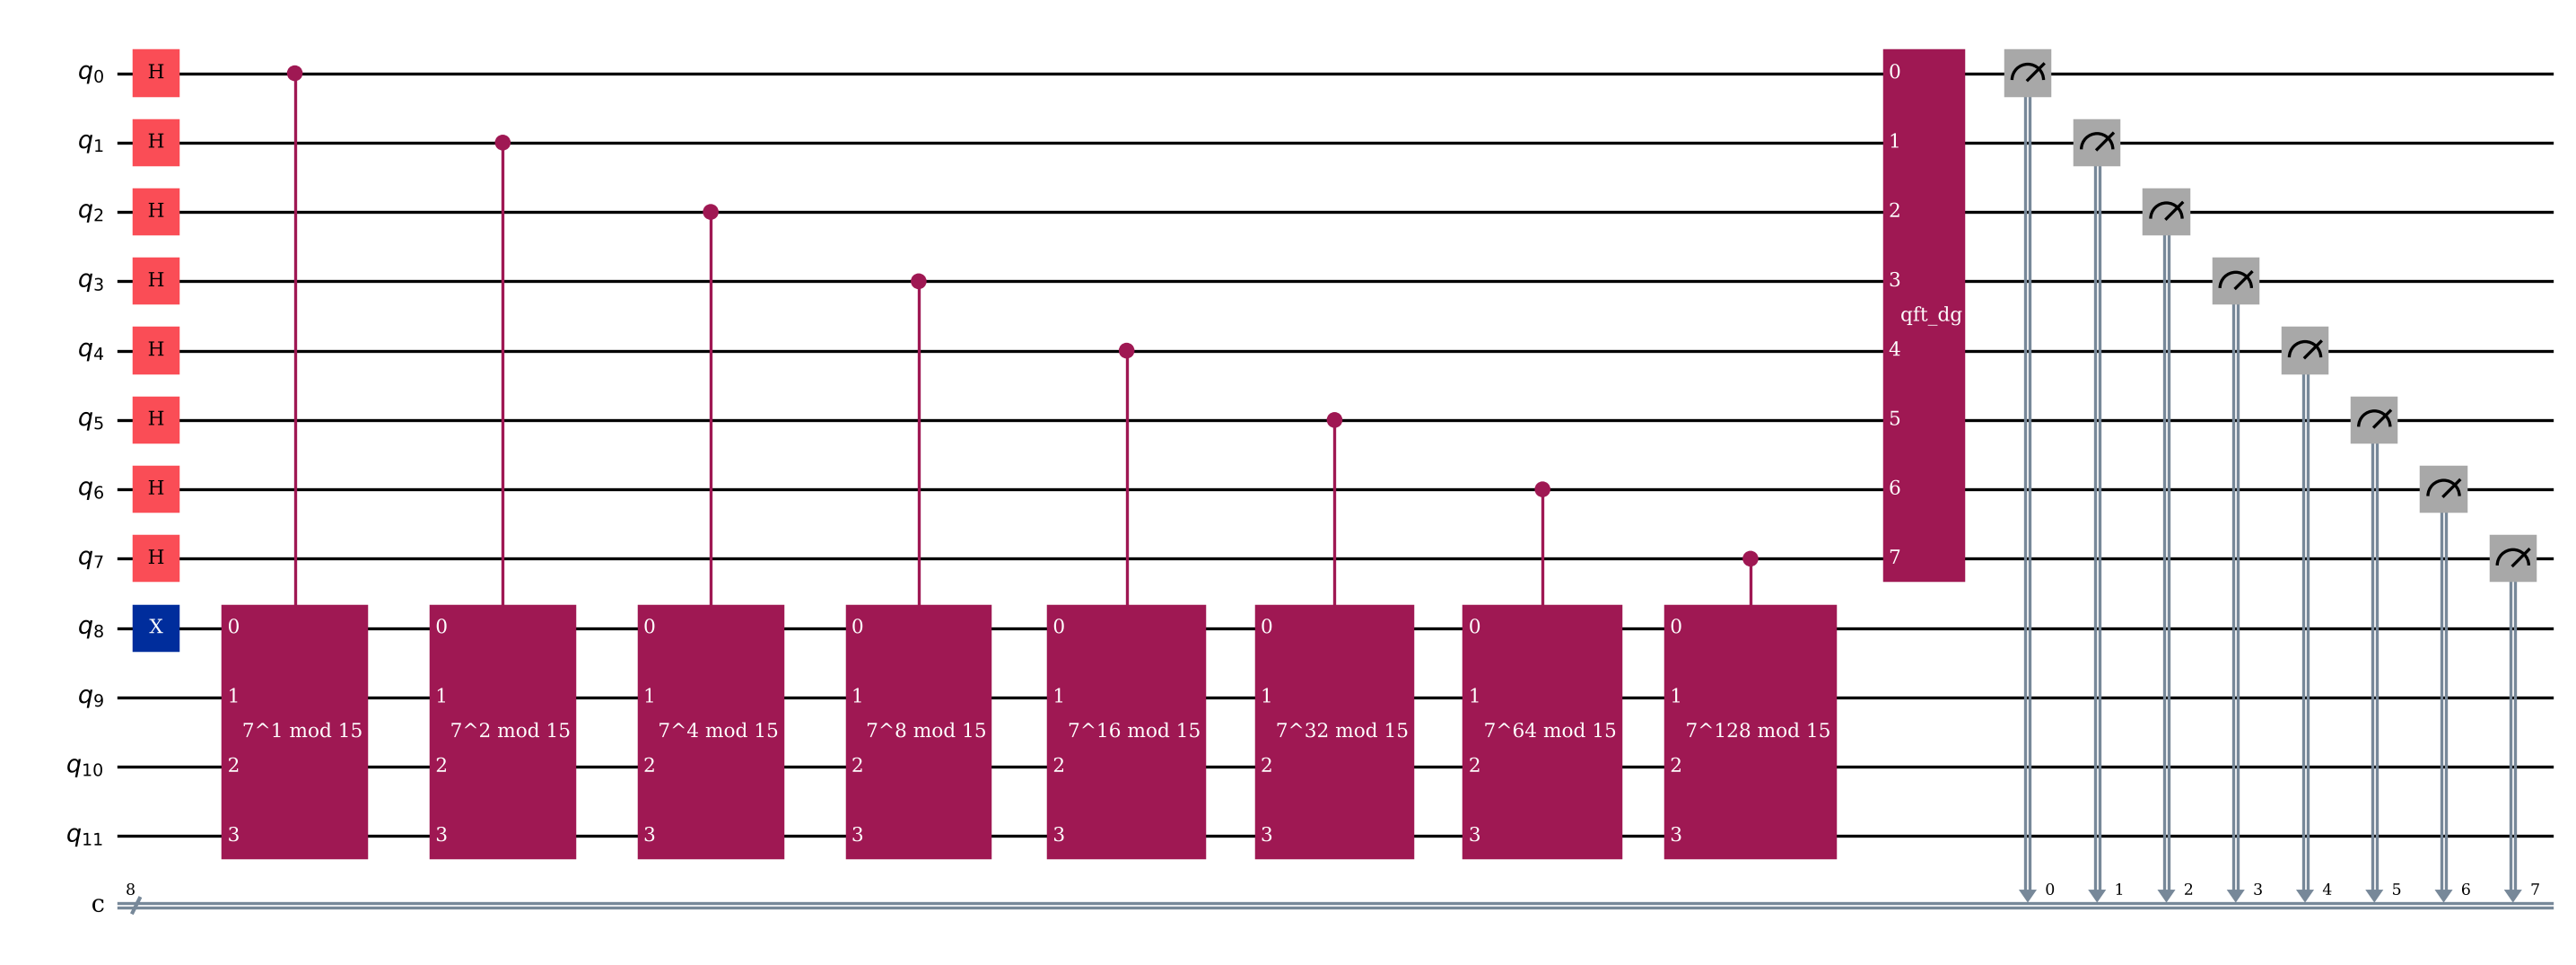
\includegraphics[width=0.82\textwidth]{assets/image3.png}\end{center}
\par

\phantomsection\label{fig:4.1}Figure 4.1: Quantum circuit for period finding ($N = 15$, $a = 7$): Hadamard gates, eight controlled modular multiplications and the inverse Quantum Fourier Transform.
\par

Figures 4.2 and 4.3 compare the simulated frequency of every outcome with its exact theoretical probability. For $N = 15$ the outcomes fall exactly on the four predicted peaks. For $N = 21$ the period is 6, which does not divide 1,024, so each peak is spread slightly over neighboring values, and the simulation reproduces that spread.
\par

\begin{center}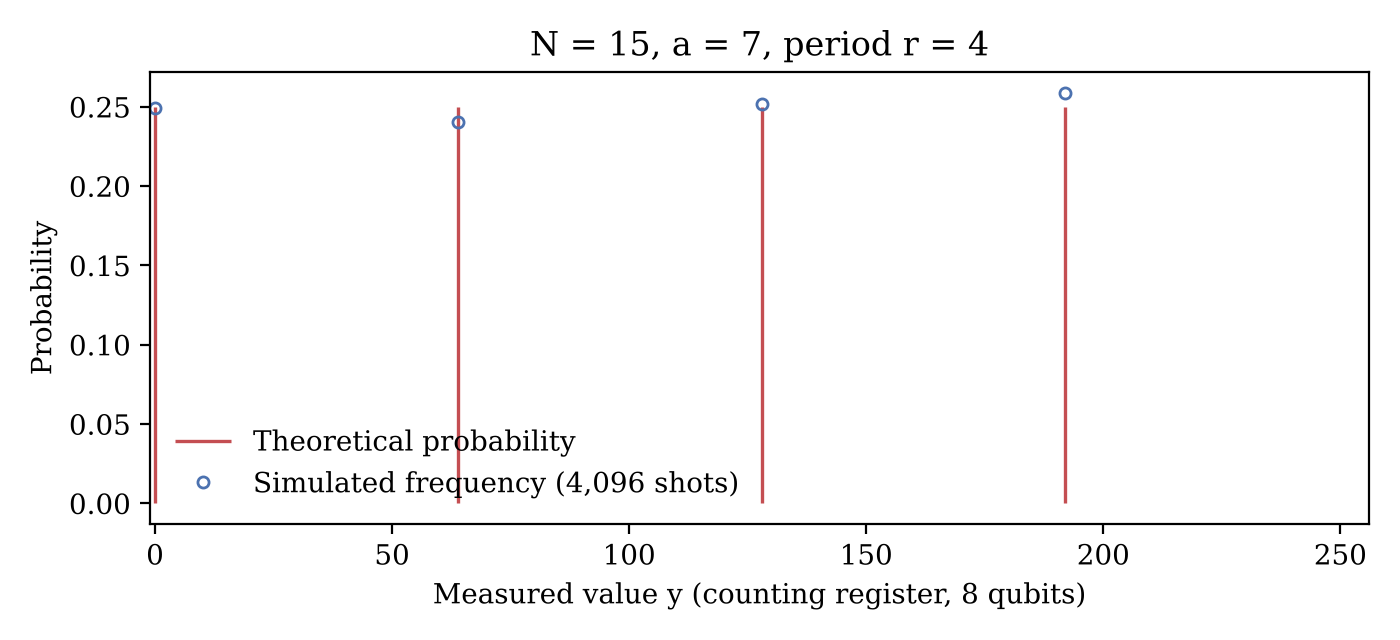
\includegraphics[width=0.82\textwidth]{assets/image4.png}\end{center}
\par

\phantomsection\label{fig:4.2}Figure 4.2: Simulated and theoretical outcome distributions for $N = 15$, $a = 7$ (period 4).
\par

\begin{center}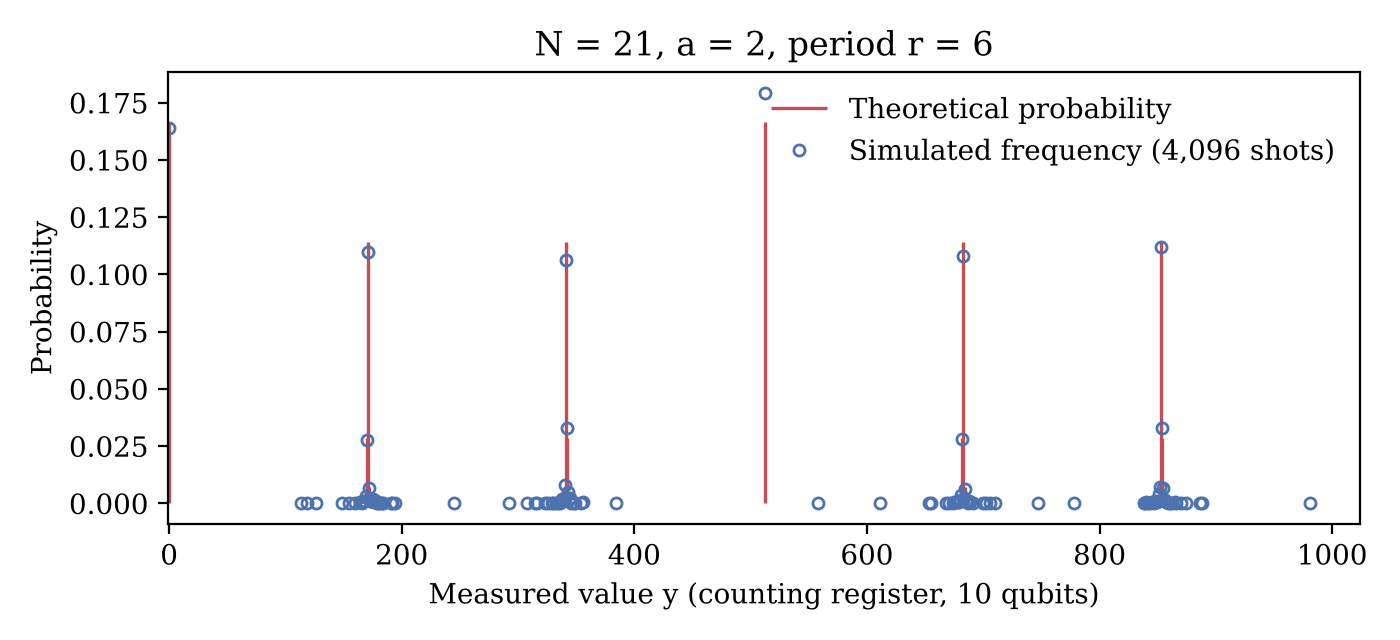
\includegraphics[width=0.82\textwidth]{assets/image5.png}\end{center}
\par

\phantomsection\label{fig:4.3}Figure 4.3: Simulated and theoretical outcome distributions for $N = 21$, $a = 2$ (period 6).
\par

\phantomsection\label{tab:4.1}Table 4.1: Observed versus theoretical success of period finding (4,096 runs per case)
\par

\begin{center}\footnotesize\begin{tabularx}{\textwidth}{|W|W|W|W|W|W|W|W|W|}\hline
N & a & r & Successful runs & Observed (\%) & Theoretical (\%) & $\chi^{2}$ (df), p & Binomial p & Factors found / reason for failure \\\hline
15 & 2 & 4 & 2,053 & 50.12 & 50.00 & 1.47 (4), 0.832 & 0.888 & $3 \times 5$ \\\hline
15 & 4 & 2 & 2,063 & 50.37 & 50.00 & 0.22 (2), 0.896 & 0.651 & $3 \times 5$ \\\hline
15 & 7 & 4 & 2,045 & 49.93 & 50.00 & 2.96 (4), 0.564 & 0.938 & $3 \times 5$ \\\hline
15 & 8 & 4 & 2,045 & 49.93 & 50.00 & 0.35 (4), 0.986 & 0.938 & $3 \times 5$ \\\hline
15 & 11 & 2 & 2,057 & 50.22 & 50.00 & 0.08 (2), 0.961 & 0.791 & $3 \times 5$ \\\hline
15 & 13 & 4 & 2,084 & 50.88 & 50.00 & 3.52 (4), 0.475 & 0.267 & $3 \times 5$ \\\hline
15 & 14 & 2 & 0 & 0.00 & 0.00 & 0.17 (2), 0.921 & — & $a^{r/2} \equiv -1 \pmod{N}$ \\\hline
21 & 2 & 6 & 1,311 & 32.01 & 32.22 & 37.06 (26), 0.074 & 0.776 & $3 \times 7$ \\\hline
21 & 4 & 3 & 0 & 0.00 & 0.00 & 17.72 (19), 0.541 & — & Odd period \\\hline
21 & 5 & 6 & 0 & 0.00 & 0.00 & 22.50 (26), 0.661 & — & $a^{r/2} \equiv -1 \pmod{N}$ \\\hline
21 & 8 & 2 & 2,120 & 51.76 & 50.00 & 5.06 (2), 0.080 & 0.025 & $3 \times 7$ \\\hline
21 & 13 & 2 & 2,071 & 50.56 & 50.00 & 0.52 (2), 0.772 & 0.482 & $3 \times 7$ \\\hline
21 & 20 & 2 & 0 & 0.00 & 0.00 & 0.17 (2), 0.921 & — & $a^{r/2} \equiv -1 \pmod{N}$ \\\hline\end{tabularx}\end{center}

\begin{center}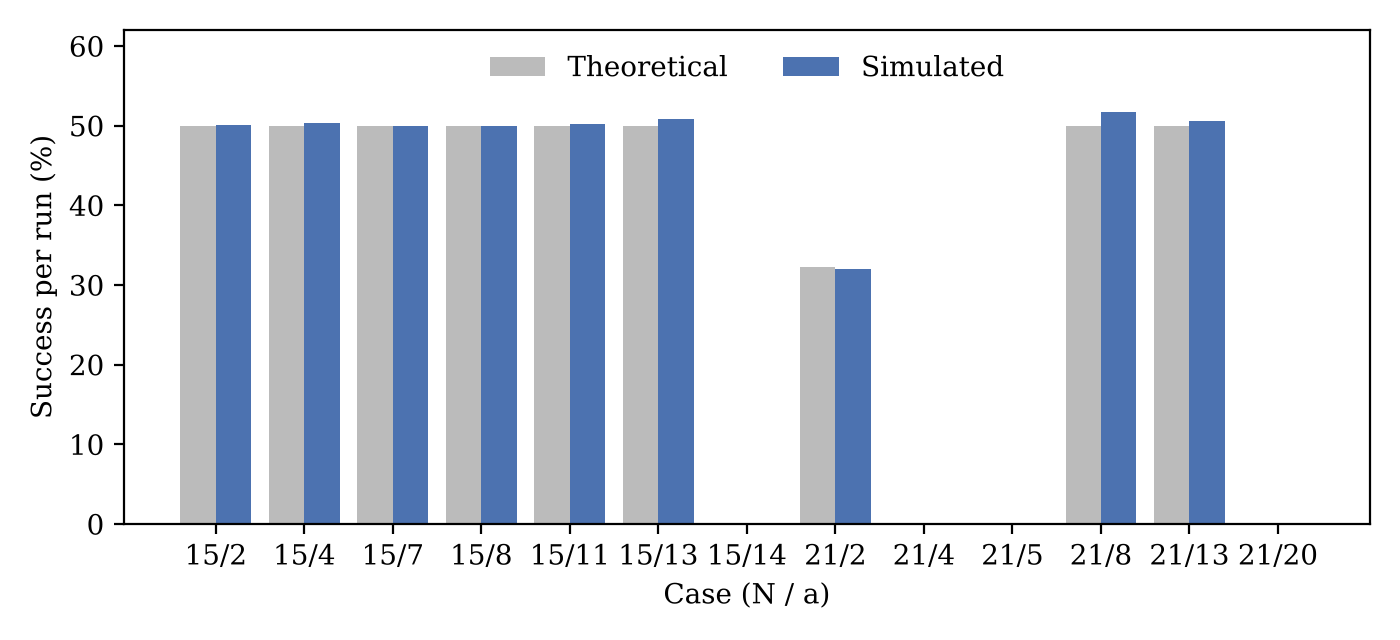
\includegraphics[width=0.82\textwidth]{assets/image6.png}\end{center}
\par

\phantomsection\label{fig:4.4}Figure 4.4: Observed and theoretical success per run for all 13 cases.
\par

Discussion. Observed success rates were within 1.8 percentage points of theory in every case. All 13 chi-square tests showed no significant difference between the simulated and theoretical outcome distributions. Of the nine binomial tests, eight gave p > 0.05; the exception, $N = 21$ with $a = 8$ ($p = 0.025$), is not significant at the Bonferroni-adjusted threshold of 0.0056, and one result below 0.05 among nine tests is consistent with chance. Fisher's method, combining all nine binomial tests, gives $\chi^{2}$ = 13.78 with 18 degrees of freedom and p = 0.744.
\par

The success rate of 32.2\% for $N = 21$, $a = 2$ is explained by the period. The six peaks correspond to fractions s/6 for $s = 0\text{ to }5$; only $s = 1$ and $s = 5$ share no factor with 6 and so reveal the full period, giving 2/6 ≈ 33.3\%, reduced slightly by the spread of peaks noted above. The four zero-success cases fail for precisely the reasons the theory predicts: an odd period ($a = 4$, $N = 21$), or $a^{r/2} \equiv -1$ ($a = 14$ for $N = 15$; $a = 5$ and $a = 20$ for $N = 21$). In those cases the quantum step still finds the period correctly, as the chi-square results show; it is the classical post-processing that cannot use it. This is why the algorithm selects a new base and repeats.
\par

\subsection*{4.3 Success Funnel and Larger Composites}
\addcontentsline{toc}{subsection}{4.3 Success Funnel and Larger Composites}

Section 1.1 distinguished period-estimation success from factor-recovery success. To make that distinction measurable, every run was traced through three stages, each of which requires the one before. A useful phase estimate is a measurement whose phase y/$2^{t}$ lies within $\frac{1}{2r^{2}}$ of some fraction s/r with $s \neq 0$; by Legendre's theorem on continued fractions, s/r is then guaranteed to appear among the convergents of y/$2^{t}$ (Hardy \& Wright, 2008). The period is recovered when the candidate from continued fractions passes the check $a^{r} \equiv 1 \pmod{N}$. The factor is recovered when that period yields a non-trivial greatest common divisor. Theoretical values come from Model A and observed values from Model B (section 3.8). The nine new cases for $N = 33$, 35 and 55 use 18-qubit circuits.
\par

\phantomsection\label{tab:4.2}Table 4.2: Success funnel for all 22 cases (observed / theoretical \%, 4,096 runs each)
\par

{\footnotesize\begin{longtable}{|P{0.08\textwidth}|P{0.04\textwidth}|P{0.12\textwidth}|P{0.12\textwidth}|P{0.12\textwidth}|P{0.13\textwidth}|P{0.09\textwidth}|P{0.19\textwidth}|}\hline
Case (N/a) & r & Useful phase & Period recovered & Factor recovered & Factor 95\% CI & Binomial p & Failure cause \\\hline
\endhead
15/2 & 4 & 75.68 / 75.00 & 50.12 / 50.00 & 50.12 / 50.00 & 48.58 – 51.66 & 0.888 &  \\\hline
15/4 & 2 & 50.37 / 50.00 & 50.37 / 50.00 & 50.37 / 50.00 & 48.82 – 51.91 & 0.650 &  \\\hline
15/7 & 4 & 75.10 / 75.00 & 49.93 / 50.00 & 49.93 / 50.00 & 48.38 – 51.47 & 0.938 &  \\\hline
15/8 & 4 & 74.80 / 75.00 & 49.93 / 50.00 & 49.93 / 50.00 & 48.38 – 51.47 & 0.938 &  \\\hline
15/11 & 2 & 50.22 / 50.00 & 50.22 / 50.00 & 50.22 / 50.00 & 48.68 – 51.76 & 0.790 &  \\\hline
15/13 & 4 & 75.24 / 75.00 & 50.88 / 50.00 & 50.88 / 50.00 & 49.34 – 52.42 & 0.267 &  \\\hline
15/14 & 2 & 49.68 / 50.00 & 49.68 / 50.00 & 0.00 / 0.00 & 0.00 – 0.09 & — & $a^{r/2} \equiv -1$ \\\hline
21/2 & 6 & 82.69 / 82.62 & 32.01 / 32.23 & 32.01 / 32.22 & 30.58 – 33.46 & 0.776 &  \\\hline
21/4 & 3 & 65.38 / 66.50 & 64.60 / 65.55 & 0.00 / 0.00 & 0.00 – 0.09 & — & Odd period \\\hline
21/5 & 6 & 81.64 / 82.62 & 32.25 / 32.23 & 0.00 / 0.00 & 0.00 – 0.09 & — & $a^{r/2} \equiv -1$ \\\hline
21/8 & 2 & 51.76 / 50.00 & 51.76 / 50.00 & 51.76 / 50.00 & 50.21 – 53.30 & 0.025 &  \\\hline
21/13 & 2 & 50.56 / 50.00 & 50.56 / 50.00 & 50.56 / 50.00 & 49.02 – 52.10 & 0.482 &  \\\hline
21/20 & 2 & 49.68 / 50.00 & 49.68 / 50.00 & 0.00 / 0.00 & 0.00 – 0.09 & — & $a^{r/2} \equiv -1$ \\\hline
33/2 & 10 & 89.62 / 89.51 & 40.45 / 39.28 & 0.00 / 0.00 & 0.00 – 0.09 & — & $a^{r/2} \equiv -1$ \\\hline
33/5 & 10 & 89.92 / 89.51 & 40.26 / 39.28 & 40.26 / 39.28 & 38.75 – 41.78 & 0.201 &  \\\hline
33/10 & 2 & 49.85 / 50.00 & 49.85 / 50.00 & 49.85 / 50.00 & 48.31 – 51.40 & 0.864 &  \\\hline
35/2 & 12 & 90.65 / 90.95 & 32.93 / 32.48 & 32.93 / 32.48 & 31.50 – 34.40 & 0.537 &  \\\hline
35/3 & 12 & 90.72 / 90.95 & 33.42 / 32.48 & 33.42 / 32.48 & 31.98 – 34.89 & 0.199 &  \\\hline
35/6 & 2 & 50.63 / 50.00 & 50.63 / 50.00 & 50.63 / 50.00 & 49.09 – 52.18 & 0.425 &  \\\hline
55/2 & 20 & 93.31 / 92.98 & 36.65 / 37.73 & 36.65 / 37.73 & 35.17 – 38.14 & 0.156 &  \\\hline
55/4 & 10 & 89.62 / 89.51 & 39.11 / 38.75 & 39.09 / 38.74 & 37.59 – 40.60 & 0.653 &  \\\hline
55/21 & 2 & 49.46 / 50.00 & 49.46 / 50.00 & 49.46 / 50.00 & 47.92 – 51.01 & 0.502 &  \\\hline\end{longtable}}

\begin{center}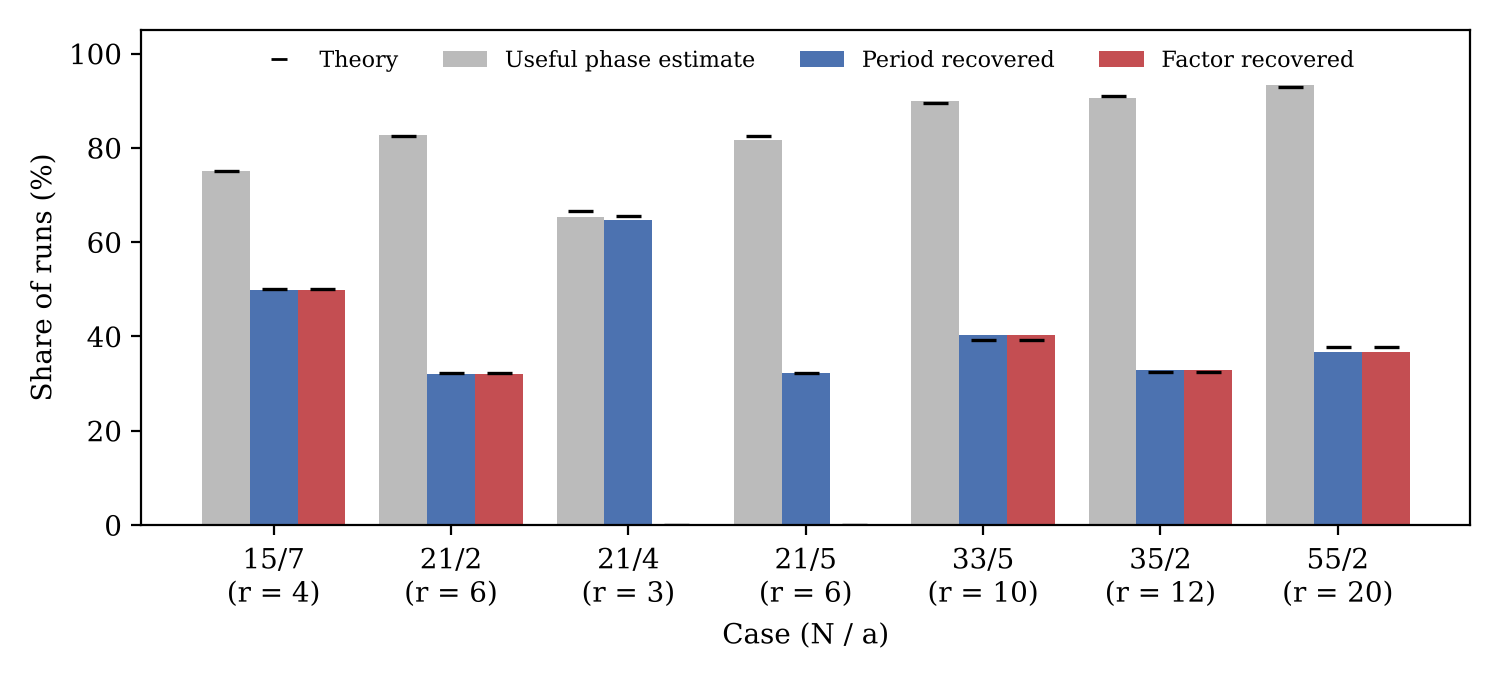
\includegraphics[width=0.82\textwidth]{assets/image7.png}\end{center}
\par

\phantomsection\label{fig:4.5}Figure 4.5: Success funnel for selected cases: useful phase estimate, period recovered and factor recovered (bars = simulation, black marks = theory).
\par

Discussion. Observed and theoretical values agreed within 1.8 percentage points at every stage in every case, and the theoretical factor-recovery rate lay inside the 95\% confidence interval in 21 of 22 cases; the exception, $N = 21$ with $a = 8$, is the same borderline case discussed in section 4.2. Across all 17 cases with a non-zero theoretical rate, the binomial tests combine by Fisher's method to $\chi^{2}$ = 29.41 with 34 degrees of freedom ($p = 0.692$).
\par

The funnel locates each loss precisely. The step from a useful phase to the period loses the runs in which s shares a factor with r, because continued fractions then return only a divisor of r. In the idealised case where r divides $2^{t}$, each measurement gives exactly $y/2^{t} = s/r$, with s equally likely to be any of $0, 1, \ldots, r-1$. Continued fractions return s/r in lowest terms, whose denominator is $r/\gcd(s, r)$, so the full period is recovered only when $\gcd(s, r) = 1$. Exactly $\varphi(r)$ values of s satisfy this, where $\varphi$ is Euler's totient function, giving
\[ P_{\text{period}} = \frac{\varphi(r)}{r}. \]
When r does not divide $2^{t}$, each peak spreads over neighbouring outcomes and the expression becomes an approximation, valid conditional on a phase estimate accurate enough for continued fractions (section 4.4). It is therefore the probability of recovering the period, not the overall success probability of Shor's algorithm: factor recovery additionally requires r to be even and $a^{r/2} \not\equiv -1 \pmod{N}$. The observed period-recovery rates follow $\varphi(r)/r$ closely: 2/6 ≈ 33\% for $r = 6$, 4/10 = 40\% for $r = 10$, 4/12 ≈ 33\% for $r = 12$ and 2/3 ≈ 67\% for $r = 3$.
\par

The step from the period to a factor loses nothing in most cases, but everything in five, each mapped to its mathematical cause in the final column of Table 4.2: the odd period of $N = 21$, $a = 4$, and the four bases with $a^{r/2} \equiv -1 \pmod{N}$, including $N = 33$, $a = 2$, where $2^{5} = 32 \equiv -1 \pmod{33}$. In these five cases the quantum measurement recovered the period in 32\% to 65\% of runs; the failure lies entirely in the number theory of the chosen base. The larger composites also show that success depends on the period, not on the size of N: $N = 55$ with $a = 21$ ($r = 2$) succeeds as often as N = 15.
\par

\subsection*{4.4 Effect of Phase-Estimation Precision}
\addcontentsline{toc}{subsection}{4.4 Effect of Phase-Estimation Precision}

Shor's algorithm uses t = 2n counting qubits so that $2^{t} \ge N^{2}$. The reason is that two distinct fractions with denominators at most N differ by at least $1/N^{2}$, so a phase measured to within $\frac{1}{2N^{2}}$ identifies a unique fraction. To test this, the three precision cases in section 3.6 were rerun with fewer counting qubits.
\par

\phantomsection\label{tab:4.3}Table 4.3: Period recovered against counting qubits (observed / theoretical \%, 4,096 runs each)
\par

\begin{center}\small\begin{tabularx}{\textwidth}{|W|W|W|W|W|}\hline
Counting qubits t & $2^{t}$ & $N = 15$, $a = 7$ ($r = 4$) & $N = 21$, $a = 2$ ($r = 6$) & $N = 35$, $a = 2$ ($r = 12$) \\\hline
2 & 4 & 49.66 / 50.00 & — & — \\\hline
3 & 8 & 51.44 / 50.00 & 0.00 / 0.00 & — \\\hline
4 & 16 & 51.15 / 50.00 & 0.00 / 0.00 & 0.00 / 0.00 \\\hline
5 & 32 & 50.66 / 50.00 & 1.27 / 1.17 & 0.00 / 0.00 \\\hline
6 & 64 & 50.07 / 50.00 & 0.56 / 0.51 & 0.00 / 0.00 \\\hline
7 & 128 & 50.63 / 50.00 & 23.05 / 22.99 & 0.00 / 0.00 \\\hline
8 & 256 & 50.81 / 50.00 & 27.95 / 28.58 & 21.92 / 22.81 \\\hline
9 & 512 & — & 30.98 / 30.88 & 28.12 / 28.52 \\\hline
10 & 1,024 & — & 31.64 / 32.23 & 28.74 / 29.93 \\\hline
11 & 2,048 & — & — & 31.91 / 31.66 \\\hline
12 & 4,096 & — & — & 31.64 / 32.48 \\\hline\end{tabularx}\end{center}

\begin{center}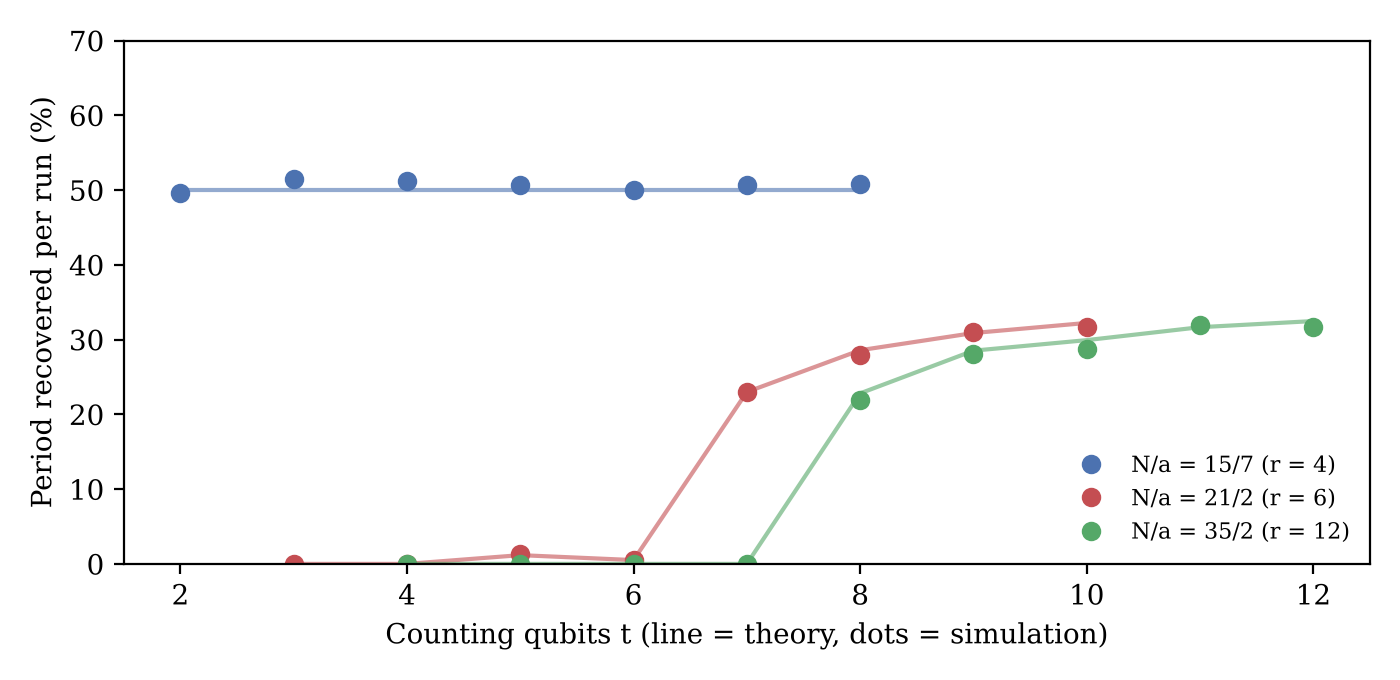
\includegraphics[width=0.82\textwidth]{assets/image8.png}\end{center}
\par

\phantomsection\label{fig:4.6}Figure 4.6: Period recovery against the number of counting qubits (lines = theory, dots = simulation).
\par

Discussion. When the period is a power of two, as for $N = 15$ with $r = 4$, the peaks fall exactly on measurable values, and the period is recovered in 50\% of runs with as few as two counting qubits. When it is not, recovery shows a sharp threshold. For $N = 35$ with $r = 12$, nothing is recovered until $t = 8$, the first value at which the resolution $1/2^{t+1}$ falls below Legendre's bound $\frac{1}{2r^{2}}$ = 1/288. For $N = 21$ with $r = 6$, Legendre's bound is already met at $t = 6$, yet recovery is only 0.5\%. At insufficient precision, the measured phase $y/2^{t}$ can lie closer to a rational number whose denominator is not the true order r, so the continued-fraction procedure may return an incorrect convergent or a proper divisor of r. At $t = 6$ the outcome 11/64 ≈ 0.172 is nearer to 3/17 than to 1/6. Recovery approaches its full value only near $t = 9$ for $N = 21$ and $t = 11$ for $N = 35$, the points at which $2^{t} \ge N^{2}$. The experiment therefore empirically supports the continued-fraction argument behind Shor's choice of register size. Because only small integers were tested, it shows consistency with that argument rather than proving it.
\par

\subsection*{4.5 Independent Verification with SymPy}
\addcontentsline{toc}{subsection}{4.5 Independent Verification with SymPy}

To make sure the results do not depend on the simulation code's own arithmetic, the key quantities were recomputed independently with SymPy (Meurer et al., 2017).
\par

\phantomsection\label{tab:4.4}Table 4.4: Independent verification with SymPy
\par

\begin{center}\footnotesize\begin{tabularx}{\textwidth}{|W|W|W|W|W|W|}\hline
N & a & r (simulation code) & r (SymPy) & Factorisation (SymPy) & Period verdicts agreeing (\%) \\\hline
15 & 2 & 4 & 4 & $3 \times 5$ & 100.00 \\\hline
15 & 4 & 2 & 2 & $3 \times 5$ & 100.00 \\\hline
15 & 7 & 4 & 4 & $3 \times 5$ & 100.00 \\\hline
15 & 8 & 4 & 4 & $3 \times 5$ & 100.00 \\\hline
15 & 11 & 2 & 2 & $3 \times 5$ & 100.00 \\\hline
15 & 13 & 4 & 4 & $3 \times 5$ & 100.00 \\\hline
15 & 14 & 2 & 2 & $3 \times 5$ & 100.00 \\\hline
21 & 2 & 6 & 6 & $3 \times 7$ & 99.54 \\\hline
21 & 4 & 3 & 3 & $3 \times 7$ & 99.56 \\\hline
21 & 5 & 6 & 6 & $3 \times 7$ & 99.44 \\\hline
21 & 8 & 2 & 2 & $3 \times 7$ & 100.00 \\\hline
21 & 13 & 2 & 2 & $3 \times 7$ & 100.00 \\\hline
21 & 20 & 2 & 2 & $3 \times 7$ & 100.00 \\\hline
33 & 2 & 10 & 10 & $3 \times 11$ & 99.73 \\\hline
33 & 5 & 10 & 10 & $3 \times 11$ & 99.66 \\\hline
33 & 10 & 2 & 2 & $3 \times 11$ & 100.00 \\\hline
35 & 2 & 12 & 12 & $5 \times 7$ & 99.66 \\\hline
35 & 3 & 12 & 12 & $5 \times 7$ & 99.61 \\\hline
35 & 6 & 2 & 2 & $5 \times 7$ & 100.00 \\\hline
55 & 2 & 20 & 20 & $5 \times 11$ & 99.32 \\\hline
55 & 4 & 10 & 10 & $5 \times 11$ & 99.49 \\\hline
55 & 21 & 2 & 2 & $5 \times 11$ & 100.00 \\\hline\end{tabularx}\end{center}

Discussion. SymPy checks the classical number theory, not the quantum distribution, which is validated by the agreement between Models A and B in sections 4.2 and 4.3. Within that scope, the multiplicative order and the factorisation matched in all 22 cases. The simulation code chooses the candidate period as the best rational approximation with denominator at most N, while SymPy uses the classical continued-fraction convergents. The two post-processing methods reached the same verdict on 99.82\% of the 90,112 simulated measurements, and on 100\% for every case with $r = 2$ or r = 4. The few disagreements occur at low-probability outcomes between peaks and would change no success rate by more than 0.7 percentage points.
\par

\subsection*{4.6 Circuit Resources}
\addcontentsline{toc}{subsection}{4.6 Circuit Resources}

Table 4.5 records the resources of each circuit (base $a = 2$) after compilation to a standard gate set of single-qubit rotations and two-qubit controlled-NOT gates.
\par

\phantomsection\label{tab:4.5}Table 4.5: Circuit resources after compilation ($a = 2$)
\par

\begin{center}\footnotesize\begin{tabularx}{\textwidth}{|W|W|W|W|W|W|W|}\hline
N & Bits n & Counting qubits & Total qubits & Two-qubit gates & Single-qubit gates & Depth \\\hline
15 & 4 & 8 & 12 & 539 & 2,965 & 1,936 \\\hline
21 & 5 & 10 & 15 & 10,145 & 58,216 & 40,233 \\\hline
33 & 6 & 12 & 18 & 49,830 & 281,040 & 196,461 \\\hline
35 & 6 & 12 & 18 & 49,830 & 281,021 & 196,452 \\\hline
55 & 6 & 12 & 18 & 49,830 & 281,092 & 196,513 \\\hline\end{tabularx}\end{center}

\begin{center}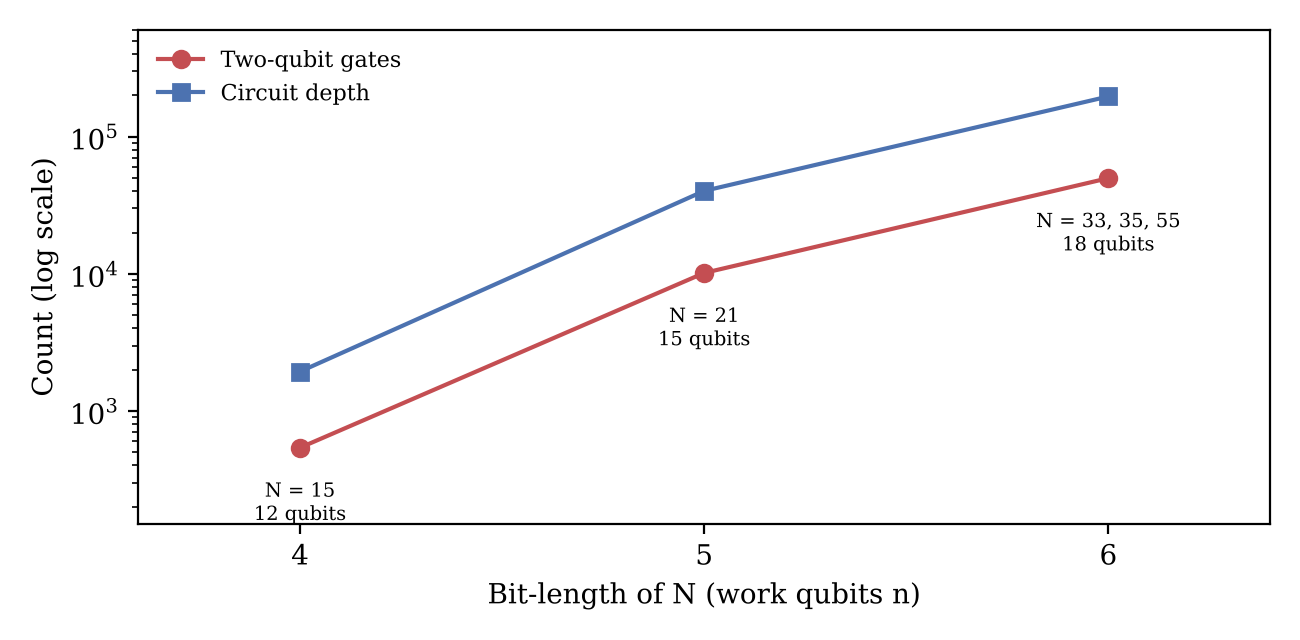
\includegraphics[width=0.82\textwidth]{assets/image9.png}\end{center}
\par

\phantomsection\label{fig:4.7}Figure 4.7: Two-qubit gate count and circuit depth against the bit-length of N.
\par

Discussion. In the implementation used in this study, the total number of qubits is 3n, because the circuit uses 2n counting qubits and n work qubits; other constructions use fewer, such as Beauregard's (2003) 2n + 3. The gate count, however, rises steeply: from 539 two-qubit gates for $N = 15$ to 10,145 for $N = 21$ and 49,830 for the 6-bit integers. $N = 33$, 35 and 55 need identical resources, because the count depends on the bit-length, not on N itself. This growth reflects the simulation method, not Shor's algorithm. Each controlled modular multiplication is built here as a general unitary operation, whose cost grows exponentially with n, whereas arithmetic circuits such as Beauregard's (2003) grow polynomially. This illustrates the scope of claims in section 3.8: the simulation demonstrates how the algorithm behaves, while its polynomial cost is a theoretical result and its cost at cryptographic scale comes from resource estimates.
\par

\subsection*{4.7 Effect of Hardware Noise}
\addcontentsline{toc}{subsection}{4.7 Effect of Hardware Noise}

The noise-free results assume perfect quantum gates. To test the effect of real hardware, the $N = 15$, $a = 7$ circuit was compiled into a standard gate set, producing 539 two-qubit gates, 2,965 single-qubit gates and a depth of 1,936 layers. It was then run under depolarising noise, with single-qubit error rates set at one tenth of the two-qubit rate.
\par

\phantomsection\label{tab:4.6}Table 4.6: Success rate under increasing gate error ($N = 15$, $a = 7$, 4,096 runs each)
\par

\begin{center}\small\begin{tabularx}{\textwidth}{|W|W|W|}\hline
Two-qubit error rate & Single-qubit error rate & Success per run (\%) \\\hline
0 (noise-free) & 0 & 50.27 \\\hline
0.01\% & 0.001\% & 47.07 \\\hline
0.03\% & 0.003\% & 45.95 \\\hline
0.1\% & 0.01\% & 42.38 \\\hline
0.3\% & 0.03\% & 36.11 \\\hline
1\% & 0.1\% & 28.69 \\\hline\end{tabularx}\end{center}

\begin{center}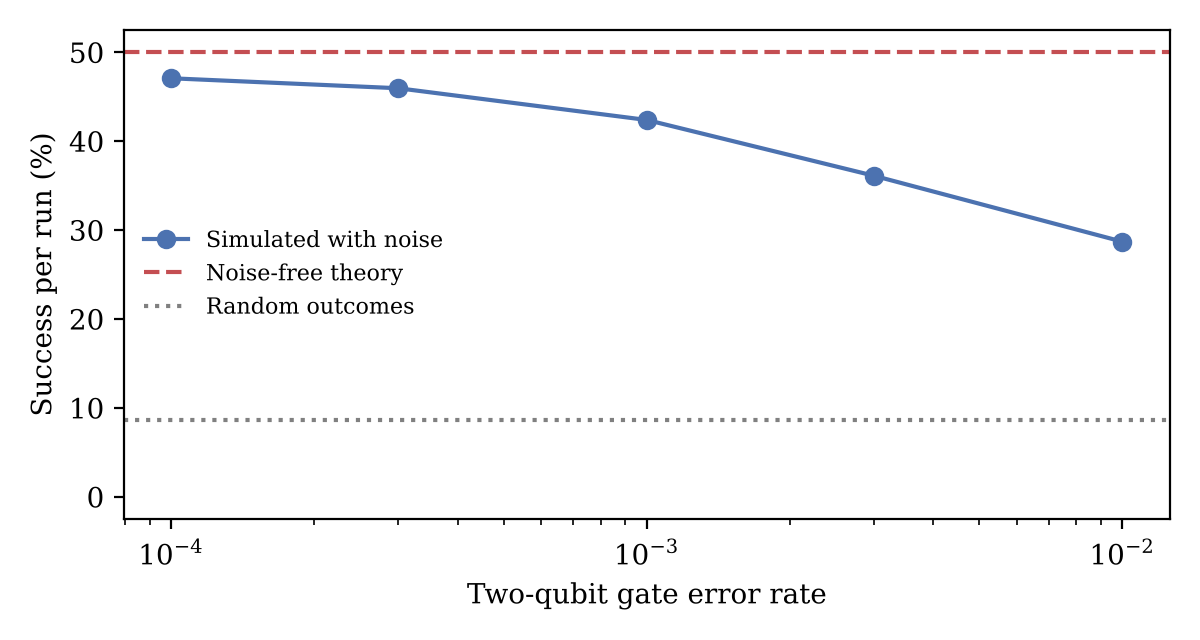
\includegraphics[width=0.82\textwidth]{assets/image10.png}\end{center}
\par

\phantomsection\label{fig:4.8}Figure 4.8: Success rate against two-qubit gate error rate, with the noise-free value and the 8.6\% rate expected from random outcomes.
\par

Discussion. Even this smallest instance needs hundreds of two-qubit gates, and success declines steadily as errors increase. In the 1\% two-qubit depolarising-error scenario, success fell by approximately 43\% relative to the noise-free simulation, although it remained well above the 8.6\% baseline for random outcomes. That baseline is the success rate if every one of the 256 possible measurement outcomes were equally likely: the post-processing recovers a factor from 22 of them, and 22/256 ≈ 8.6\%. These figures describe the noise model, not a particular device, because the model omits correlated errors, crosstalk and measurement errors; section 4.8 reports what real devices achieved. Because the circuit used here is a general compilation rather than a hand-optimised one, the gate count is higher than in specialised demonstrations; the trend, however, is what matters. Scaled to a 2048-bit modulus, the number of gates grows by many orders of magnitude, and errors compound accordingly. This is why attacks on real cryptography require error-corrected logical qubits, and why resource estimates are expressed in millions of physical qubits (Gidney \& Ekerå, 2021; Gidney, 2025). The recent demonstration of error correction below threshold (Google Quantum AI and Collaborators, 2025) addresses exactly this barrier.
\par

\subsection*{4.8 Demonstrations on IBM Quantum Hardware}
\addcontentsline{toc}{subsection}{4.8 Demonstrations on IBM Quantum Hardware}

To test whether the behaviour established in simulation survives on physical devices, five experiments were run on three 156-qubit IBM Heron superconducting processors between 14 and 16 November 2026, accessed through the IBM Quantum Platform under the Open Plan (Table 4.7). Each run used 4,096 shots and no error mitigation. Two design choices distinguish these circuits from the simulations of sections 4.2 to 4.7. First, the general construction used there compiles to hundreds of two-qubit gates even for $N = 15$ (section 4.7), more than current hardware can execute faithfully, so a smaller circuit was built for each experiment. Second, the powers $a^{2^{j}} \bmod N$ were computed classically, as in every implementation of the algorithm.
\par

The first experiment repeats the worked example $N = 15$, $a = 7$ on two devices. Because $15 = 2^{4} - 1$, multiplication modulo 15 reduces to permutations of the work qubits, which were built from controlled-SWAP and CNOT gates. Three counting qubits suffice, because the period $r = 4$ divides $2^{3} = 8$, so the ideal measurement peaks fall exactly on the outcomes 0, 2, 4 and 6.
\par

The second experiment targets a period that does not divide $2^{t}$. The integers $N = 21$ with $a = 2$ and $N = 77 = 7 \times 11$ with $a = 12$ both have period $r = 6$. With $t = 9$ counting qubits, theory predicts six peaks spread over neighbouring outcomes (section 4.4). The circuit is compiled: the work register stores the exponent index k of $a^{k} \bmod N$, and each controlled step adds $2^{j} \bmod 6$ to it. Because the circuit then depends only on r, a single hardware run serves both integers, and only the classical post-processing differs. A first version, with general controlled adders and the standard inverse Quantum Fourier Transform, compiled to 302 two-qubit gates at depth 860. A redesigned version used two mathematical simplifications. By the Chinese Remainder Theorem, $\mathbb{Z}_{6} \cong \mathbb{Z}_{2} \times \mathbb{Z}_{3}$, so the work register was split into one qubit for $k \bmod 2$ and two qubits for $k \bmod 3$; adding 2 or 4 modulo 6 then changes only the $\mathbb{Z}_{3}$ part. The semi-classical inverse Fourier transform (Griffiths \& Niu, 1996) measures the counting qubits one at a time and replaces the transform's two-qubit phase gates with single-qubit rotations chosen from earlier results, which requires mid-circuit measurement and classical feed-forward (a dynamic circuit). The redesigned circuit needed 73 two-qubit gates at depth 324. As a simple error check, the $\mathbb{Z}_{3}$ register was also measured at the end: its bit pattern 11 cannot occur in an error-free run, so shots showing it can be discarded (post-selection).
\par

\phantomsection\label{tab:4.7}Table 4.7: IBM Quantum hardware runs (4,096 shots each)
\par

\begin{center}\small\begin{tabularx}{\textwidth}{|P{0.06\textwidth}|W|W|W|P{0.09\textwidth}|P{0.12\textwidth}|P{0.08\textwidth}|}\hline
Run & Device & Date & Circuit & Qubits & Two-qubit gates & Depth \\\hline
A & ibm\_fez & 14 Nov 2026 & $N = 15$, $a = 7$ & 7 & 84 & 214 \\\hline
B & ibm\_marrakesh & 16 Nov 2026 & $N = 15$, $a = 7$ & 7 & 86 & 228 \\\hline
C & ibm\_marrakesh & 16 Nov 2026 & $r = 6$, first version & 12 & 302 & 860 \\\hline
D & ibm\_marrakesh & 16 Nov 2026 & $r = 6$, CRT and semi-classical QFT & 12 & 73 & 324 \\\hline
E & ibm\_kingston & 16 Nov 2026 & $r = 6$, CRT and semi-classical QFT & 12 & 73 & 326 \\\hline\end{tabularx}\end{center}

{\sloppy IBM job identifiers: A, \texttt{dbrqrm6jjaos73ajeil0}; B, \texttt{dbt4k17q0h0s73bkb470}; C, \texttt{dbt4c9nasvbs73b9a290}; D, \texttt{dbt4vt7q0h0s73bkbnv0}; E, \texttt{dbtbcgreq3sc73evjslg}. Runs D and E also contained 36 classically conditioned operations from the feed-forward steps.\par}

\textbf{Results for N = 15.} Table 4.8 and Figure 4.9 compare runs A and B with theory.
\par

\phantomsection\label{tab:4.8}Table 4.8: Hardware results for $N = 15$, $a = 7$ (runs A and B; random guessing is 2 of the 8 outcomes of the 3-qubit register)
\par

\begin{center}\small\begin{tabularx}{\textwidth}{|W|W|W|W|W|}\hline
Measure & Ideal theory & ibm\_fez (A) & ibm\_marrakesh (B) & Random guessing \\\hline
Success per shot (\%) & 50.00 & 45.78 (95\% CI 44.24–47.32) & 40.65 (95\% CI 39.14–42.17) & 25.00 \\\hline
Shots on predicted outcomes (\%) & 100.00 & 95.61 & 92.55 & 50.00 \\\hline
Total variation distance from ideal & 0 & 0.046 & 0.094 & 0.500 \\\hline
Classical fidelity with ideal & 1.000 & 0.956 & 0.922 & 0.500 \\\hline\end{tabularx}\end{center}

\begin{center}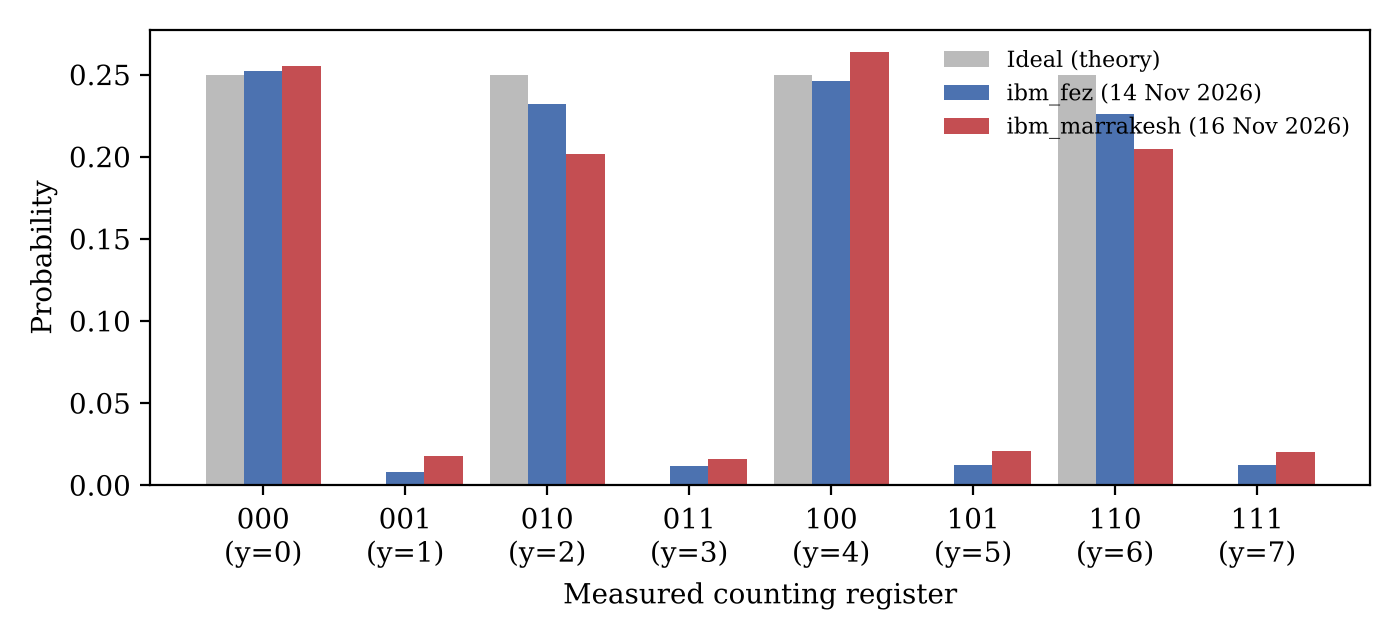
\includegraphics[width=0.82\textwidth]{assets/image12.png}\end{center}
\par

\phantomsection\label{fig:4.9}Figure 4.9: Measured distributions for $N = 15$, $a = 7$ on ibm\_fez and ibm\_marrakesh, compared with theory.
\par

Discussion. Both devices reproduced the four-peak structure predicted by the Quantum Fourier Transform: 95.6\% and 92.6\% of shots fell on the outcomes 0, 2, 4 and 6, and the remainder was spread almost evenly over the four outcomes that should never occur, the signature of device noise rather than systematic error. The outcomes 2 and 6 give the period $r = 4$, and the greatest-common-divisor step then returns the factors 3 and 5, recovered in 1,875 shots on ibm\_fez and 1,665 on ibm\_marrakesh. Both success rates are far above the 25\% expected from random outcomes (one-sided binomial tests, $p \approx 4 \times 10^{-182}$ and $p \approx 9 \times 10^{-107}$) and significantly below the ideal 50\% ($p \approx 7 \times 10^{-8}$ and $p \approx 4 \times 10^{-33}$), so device noise is measurable even for a circuit of about 85 two-qubit gates. ibm\_fez outperformed ibm\_marrakesh by 5.1 percentage points (two-proportion z-test, $z = 4.68$, $p \approx 3 \times 10^{-6}$), consistent with its lower median two-qubit error as reported by the IBM service (0.0024 against 0.0027). The ibm\_fez result lies within 1.5 percentage points of the 47.27\% predicted beforehand by a simulated noise model of that device. Because shots are independent, repeating the procedure until a factor appears succeeds with probability $1 - (1 - p)^{k}$: about 95\% (ibm\_fez) and 93\% (ibm\_marrakesh) after five repetitions.
\par

\textbf{Results for period 6.} Table 4.9 and Figure 4.10 compare the two versions of the period-6 circuit on ibm\_marrakesh, and the redesigned version on ibm\_kingston.
\par

\phantomsection\label{tab:4.9}Table 4.9: Hardware results for period 6 ($N = 21$, $a = 2$ and $N = 77$, $a = 12$; runs C, D and E)
\par

\begin{center}\small\begin{tabularx}{\textwidth}{|W|W|W|W|W|W|}\hline
Measure & Ideal theory & First version, ibm\_marrakesh (C) & Redesigned, ibm\_marrakesh (D) & Redesigned, ibm\_kingston (E) & Random guessing \\\hline
Factor success, $N = 21$ (\%) & 30.87 & 4.49 (95\% CI 3.88–5.17) & 8.50 (95\% CI 7.66–9.39) & 11.16 (95\% CI 10.21–12.16) & 5.08 \\\hline
Factor success, $N = 77$ (\%) & 22.82 & 4.05 (95\% CI 3.47–4.70) & 6.01 (95\% CI 5.30–6.78) & 7.89 (95\% CI 7.08–8.75) & 4.30 \\\hline
Factor success after post-selection, $N = 21$ / $N = 77$ (\%) & — & — & 8.87 / 6.42 & 11.49 / 8.34 & — \\\hline
Shots within ±1 of the six peaks (\%) & 93.18 & 5.22 & 17.09 & 28.30 & 3.52 \\\hline
Classical fidelity with ideal & 1.000 & 0.110 & 0.246 & 0.375 & 0.089 \\\hline\end{tabularx}\end{center}

\begin{center}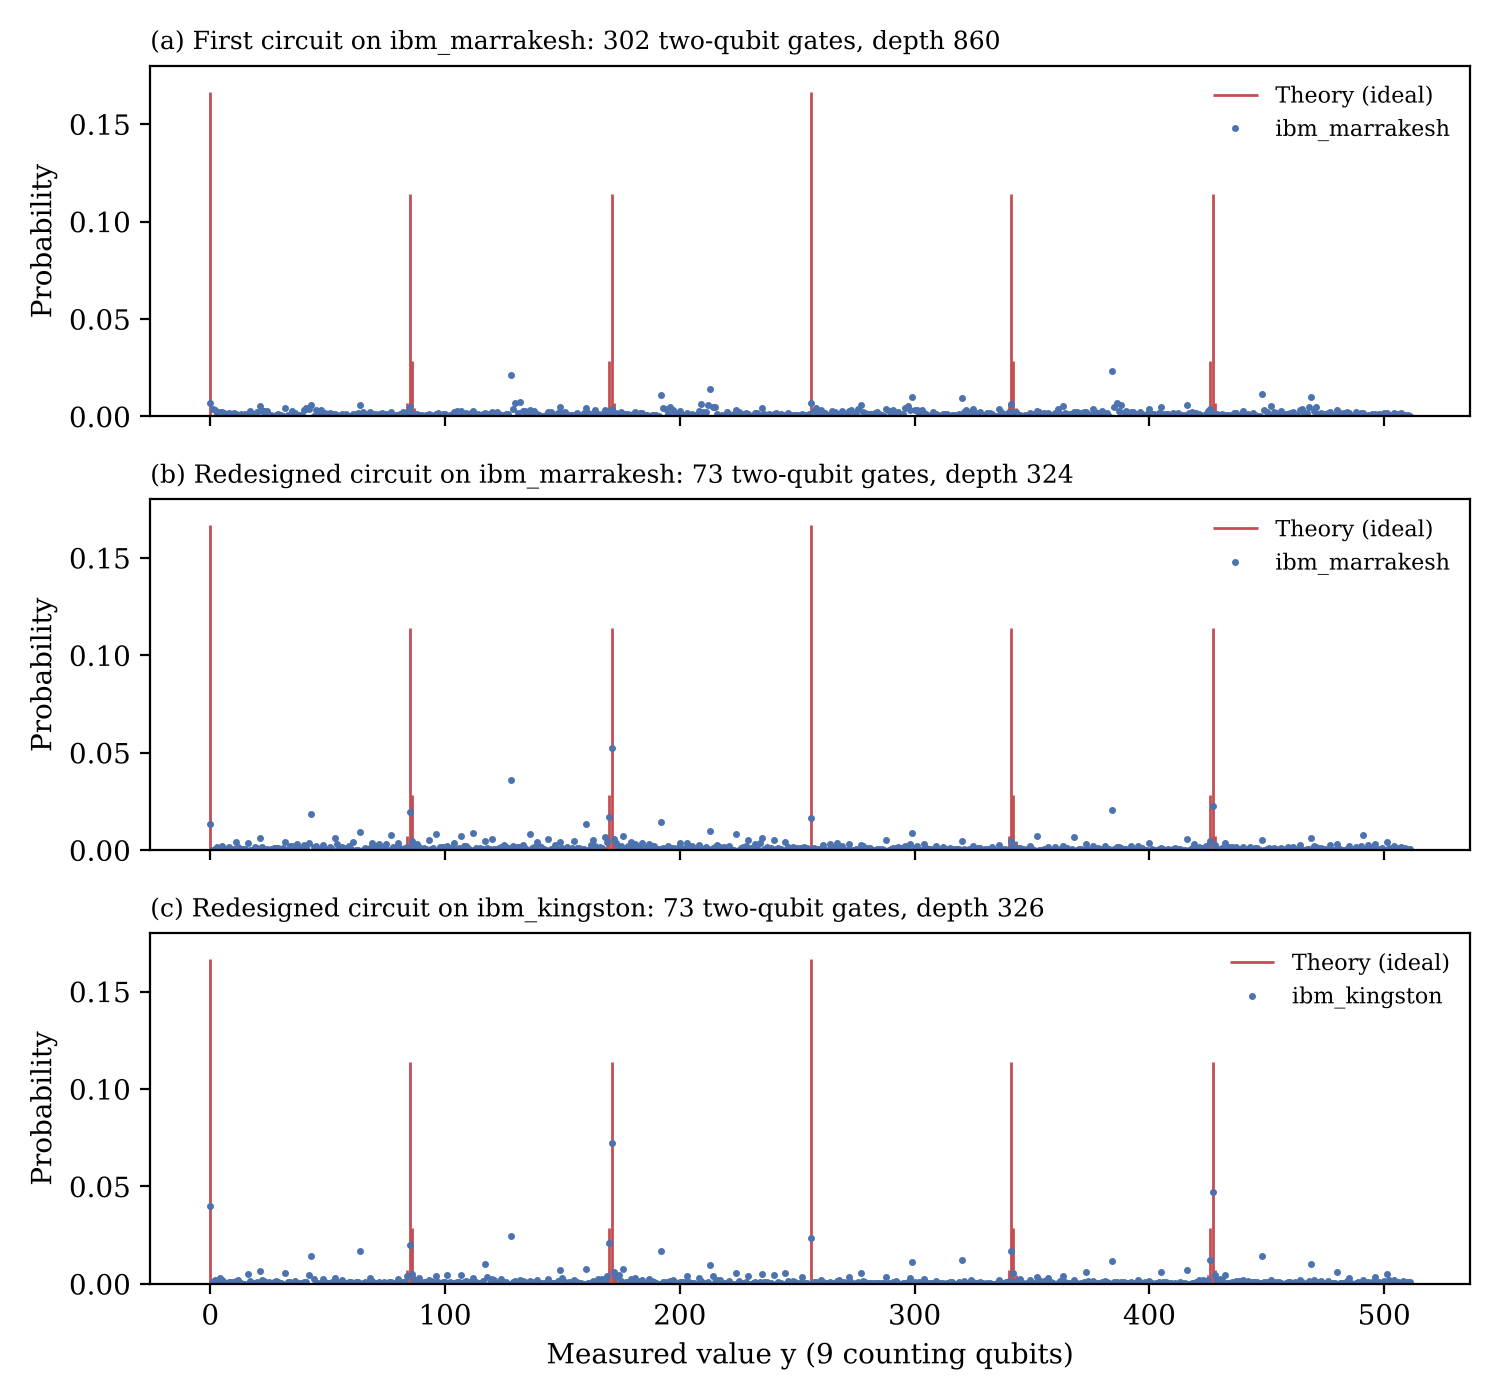
\includegraphics[width=0.82\textwidth]{assets/image13.png}\end{center}
\par

\phantomsection\label{fig:4.10}Figure 4.10: Measured distributions for the period-6 circuit: (a) first version on ibm\_marrakesh, 302 two-qubit gates; (b) redesigned version on ibm\_marrakesh, 73 two-qubit gates; (c) redesigned version on ibm\_kingston. Red lines show the theoretical distribution.
\par

Discussion. The first version lost the signal entirely: the six theoretical peaks are absent, and its success rates are statistically indistinguishable from random outcomes ($p = 0.96$ for $N = 21$). The redesigned circuit restored a statistically significant signal. For $N = 21$, success was 1.7 times the random baseline (one-sided binomial test, $p \approx 4 \times 10^{-20}$); for $N = 77$ the gain was smaller but still significant ($p \approx 2 \times 10^{-7}$). The share of shots near the theoretical peaks rose from 5.2\% to 17.1\%, against 3.5\% for random outcomes. Post-selection discarded the 12.5\% of shots with the impossible $\mathbb{Z}_{3}$ pattern and raised success only modestly, to 8.87\% and 6.42\%. On ibm\_kingston the same redesigned circuit performed better still: 11.16\% success for $N = 21$, 2.2 times the random baseline ($p \approx 8 \times 10^{-54}$), and 7.89\% for $N = 77$ ($p \approx 1 \times 10^{-24}$), with 28.3\% of shots near the theoretical peaks. The improvement over ibm\_marrakesh is statistically significant (two-proportion z-tests, $p \approx 5 \times 10^{-5}$ for $N = 21$ and $p \approx 8 \times 10^{-4}$ for $N = 77$) and matches the ordering of the devices' median two-qubit errors as reported by the IBM service (0.0019 for ibm\_kingston against 0.0027 for ibm\_marrakesh), the same ordering by device quality seen for $N = 15$. Performance on both devices nevertheless remained far below the ideal 30.9\%, and on ibm\_marrakesh below the 26.7\% predicted beforehand by a simulated noise model of that device.
\par

The redesigned runs also show how the signal degrades, and the pattern is the same on both devices. The peak at phase 2/6 (outcome 171) was strongest, at 7.5\% (ibm\_marrakesh) and 9.9\% (ibm\_kingston) of shots within one outcome of it against 15.0\% ideally, while the peaks at phases 0 and 1/2 (outcomes 0 and 256) were weakest, at 1.4\% and 1.8\% on ibm\_marrakesh and 4.2\% and 2.5\% on ibm\_kingston, against 16.7\%. Because the pattern repeats on two processors, it is more likely a property of the circuit design than of either device. The most significant bits of the result were the most degraded. This is consistent with the semi-classical design, in which the qubit carrying the most significant bit is measured last: it idles through eight rounds of mid-circuit measurement and feed-forward and inherits any errors in the earlier corrections. This is a plausible explanation rather than a demonstrated one, since confirming it would require device-level characterisation. All three period-6 runs also show excess counts at multiples of 64 (for example outcomes 128, 192, 320, 384 and 448), between 3 and 18 times the level expected from uniform noise. Because this appears on both devices and with both circuit versions, it is not a device-specific artefact; its cause is not investigated here. Dynamical decoupling, which protects idle qubits, could not be applied, because the IBM service does not support it for circuits with mid-circuit feed-forward.
\par

Four conclusions follow. First, circuit size decides whether a signal survives: about 85 two-qubit gates preserved the structure predicted by theory, while 302 destroyed it. Second, the two-qubit gate count is not a sufficient measure of difficulty. Runs D and E needed fewer two-qubit gates than runs A and B yet performed far worse, because a dynamic circuit trades gates for mid-circuit measurement and waiting time, during which idle qubits decohere. The simulated noise models, which under-represent these effects, overestimated performance for both period-6 runs. Third, identical quantum data give different success rates for different N: the same measurements recovered factors of 21 more often than factors of 77 (8.5\% against 6.0\%), because the continued-fraction step must rule out more competing fractions with denominators up to 77, as section 4.4 predicts; the same held on ibm\_kingston (11.2\% against 7.9\%). Fourth, device quality matters: for both circuits run on more than one processor, the device with the lower median two-qubit error performed significantly better.
\par

These demonstrations have clear limits. The $N = 15$ circuit relies on the special structure of multiplication modulo 15, and the period-6 circuit encodes the period it seeks, so the runs demonstrate phase estimation and post-processing on real hardware, not a general factoring capability. Simplified circuits of this kind are known to overstate what a demonstration establishes (Smolin et al., 2013). Each experiment was run once, under the calibration in effect at the time. The results show where present hardware stands for very small instances; they do not indicate progress towards factoring cryptographic moduli, which would require large numbers of error-corrected logical qubits (section 2.4).
\par

\subsection*{4.9 Quantum Exposure of Payment Cryptography (Objective 3)}
\addcontentsline{toc}{subsection}{4.9 Quantum Exposure of Payment Cryptography (Objective 3)}

Shor's algorithm breaks public-key schemes completely: increasing the key size does not restore security, because the attack cost grows only polynomially with key length. Grover's algorithm only shortens the effective key length of symmetric ciphers, by at most half in the ideal case. Table 4.10 quantifies the second effect. NIST frames its post-quantum security levels around the maximum circuit depth an attacker can run, between $2^{40}$ and $2^{96}$ sequential steps (NIST, 2016). Because Grover's algorithm parallelises poorly, a depth cap forces the attacker to split the search across many machines, which sharply increases the total work.
\par

\phantomsection\label{tab:4.10}Table 4.10: Grover key-search cost for AES ($\log_{2}$ of Grover iterations)
\par

\begin{center}\footnotesize\begin{tabularx}{\textwidth}{|W|W|W|W|W|W|W|}\hline
Algorithm & Classical security (bits) & Ideal quantum security (bits) & Iterations, unlimited depth & Total, depth $\le 2^{40}$ & Total, depth $\le 2^{64}$ & Total, depth $\le 2^{96}$ \\\hline
AES-128 & 128 & 64 & 63.7 & 87.3 & 63.7 & 63.7 \\\hline
AES-192 & 192 & 96 & 95.7 & 151.3 & 127.3 & 95.7 \\\hline
AES-256 & 256 & 128 & 127.7 & 215.3 & 191.3 & 159.3 \\\hline\end{tabularx}\end{center}

These figures count Grover iterations only. Each iteration requires a full quantum implementation of AES, costing thousands of additional gates (Grassl et al., 2016; Jaques et al., 2020), so real costs are higher still. Under the strictest depth limit, an attack on AES-128 needs about $2^{87}$ iterations in total, far above the idealised $2^{64}$. AES-256 stays above $2^{127}$ iterations in every scenario. Under the resource and depth assumptions considered here, this supports the conclusion that Grover's algorithm only reduces the security margin of a well-designed symmetric cipher, and that AES-256 retains a substantial margin against generic Grover search. These are resource-based conclusions, not mathematical guarantees. The qualification is that some symmetric constructions can be attacked more strongly if an adversary can query them in quantum superposition (Kaplan et al., 2016); this does not apply to generic key search against AES.
\par

\phantomsection\label{tab:4.11}Table 4.11: Quantum exposure of payment-system components
\par

\begin{center}\small\begin{tabularx}{\textwidth}{|W|W|W|W|}\hline
Component & Cryptography & Exposure & Remedy \\\hline
HSM remote key loading / key transport & RSA & Broken & Replace with ML-KEM \\\hline
TLS key exchange (gateways, APIs) & ECDHE / RSA & Broken & Replace with ML-KEM (hybrid during transition) \\\hline
EMV offline data authentication & RSA & Broken & Replace with post-quantum signatures (e.g. ML-DSA) \\\hline
TLS / PKI certificates & RSA / ECDSA & Broken & Replace with ML-DSA at certificate renewal \\\hline
Tokenisation vault and token cryptograms & AES & Weakened & Use AES-256 \\\hline
EMV online authorisation cryptogram (ARQC) & 3DES / AES & Weakened & Retire 3DES; use AES-256 card keys \\\hline
PIN block encryption & 3DES / AES & Weakened & Retire 3DES; use AES PIN blocks \\\hline\end{tabularx}\end{center}

Discussion. A key finding is the split within EMV itself. Online authorisation relies on symmetric keys shared between the card and its issuer, so it is largely quantum-resistant once 3DES is retired. Offline data authentication relies on RSA certificates, making it the quantum-vulnerable element of the chip ecosystem, consistent with EMVCo's assessment (EMVCo, 2025). The remedies also differ in kind: symmetric components need a key-length change within an existing algorithm, while public-key components need new algorithms, larger keys and signatures, and changes to specifications, hardware and certification.
\par

\subsection*{4.10 Migration Priority Ranking (Objective 4)}
\addcontentsline{toc}{subsection}{4.10 Migration Priority Ranking (Objective 4)}

Table 4.12 applies the scoring method of section 3.5 to the most likely values in Table 3.3. Figure 4.11 shows each component's combined shelf life and migration time against the three threat scenarios.
\par

\phantomsection\label{tab:4.12}Table 4.12: Migration priority scores and ranking (most likely values)
\par

\begin{center}\footnotesize\begin{tabularx}{\textwidth}{|W|W|W|W|W|W|W|}\hline
Rank (central) & Component & Exposure & $x + y$ (years) & Score, near (2032) & Score, central (2035) & Score, late (2040) \\\hline
1 & HSM remote key loading / key transport & Broken & 17 & 11.0 & 8.0 & 3.0 \\\hline
2 & EMV offline data authentication & Broken & 14 & 8.0 & 5.0 & 0.0 \\\hline
3 & TLS key exchange (gateways, APIs) & Broken & 11 & 5.0 & 2.0 & $-3.0$ \\\hline
4 & Tokenisation vault and token cryptograms & Weakened & 13 & 2.1 & 1.2 & $-0.3$ \\\hline
5 & PIN block encryption & Weakened & 10 & 1.2 & 0.3 & $-1.2$ \\\hline
6 & EMV online authorisation cryptogram (ARQC) & Weakened & 7 & 0.3 & $-0.6$ & $-2.1$ \\\hline
7 & TLS / PKI certificates & Broken & 6 & 0.0 & $-3.0$ & $-8.0$ \\\hline\end{tabularx}\end{center}

\begin{center}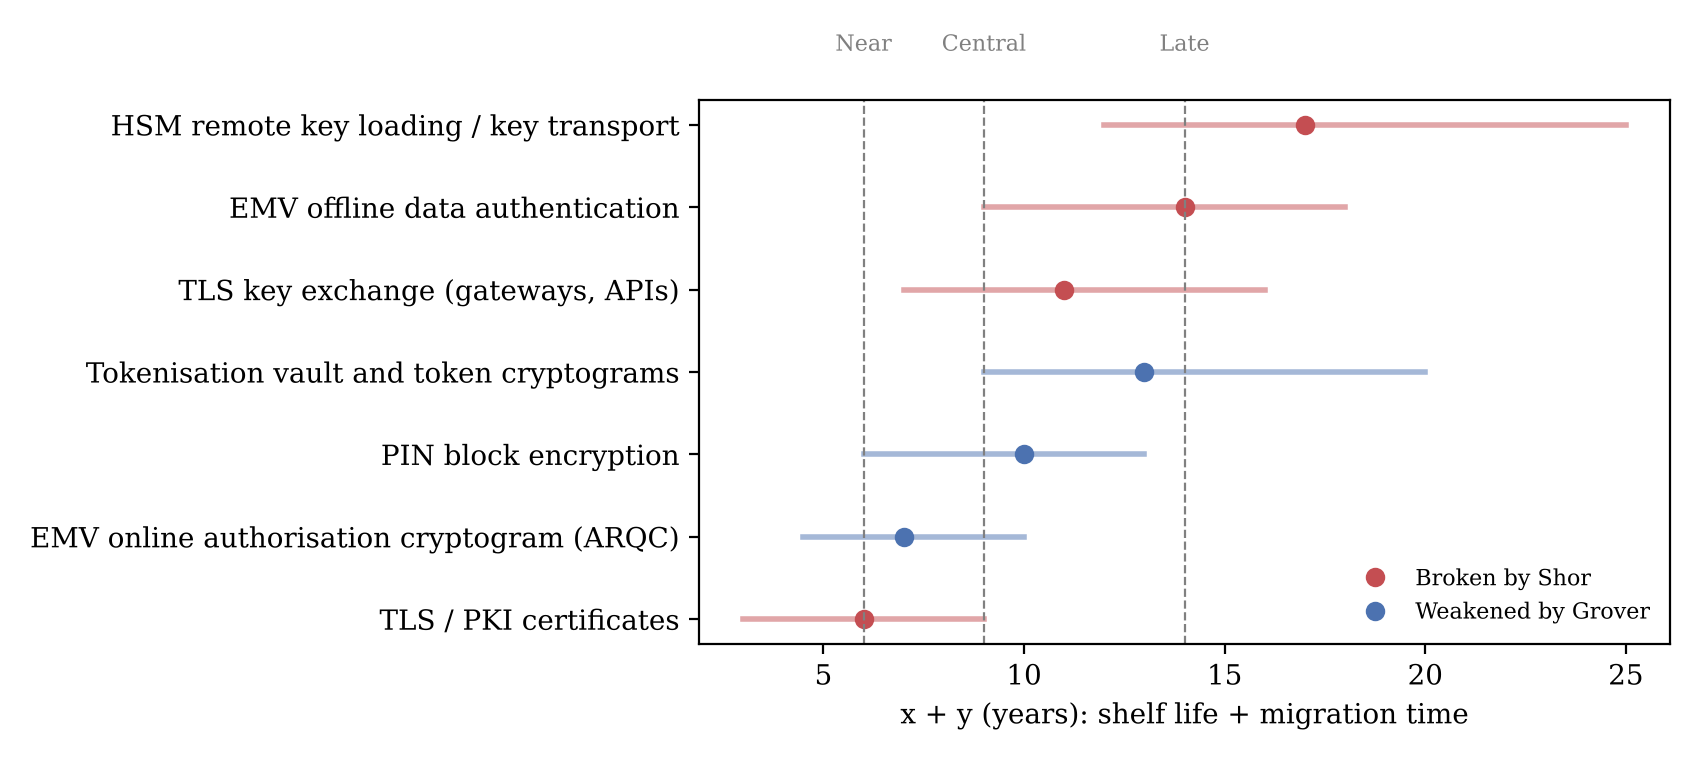
\includegraphics[width=0.82\textwidth]{assets/image11.png}\end{center}
\par

\phantomsection\label{fig:4.11}Figure 4.11: Shelf life plus migration time for each component (dot = most likely value, bar = low-to-high range) against the near, central and late threat scenarios.
\par

To test how far the ranking depends on the estimated parameters, x and y were drawn 20,000 times from triangular distributions spanning the low, most likely and high values in Table 3.3.
\par

\phantomsection\label{tab:4.13}Table 4.13: Monte Carlo sensitivity analysis (20,000 draws)
\par

\begin{center}\footnotesize\begin{tabularx}{\textwidth}{|W|W|W|W|W|W|}\hline
Component & P(at risk), near & P(at risk), central & P(at risk), late & P(top-3 priority), central & Median rank, central \\\hline
HSM remote key loading / key transport & 1.000 & 1.000 & 0.989 & 1.000 & 1 \\\hline
EMV offline data authentication & 1.000 & 1.000 & 0.409 & 0.990 & 2 \\\hline
TLS key exchange (gateways, APIs) & 1.000 & 0.967 & 0.023 & 0.712 & 3 \\\hline
Tokenisation vault and token cryptograms & 1.000 & 1.000 & 0.480 & 0.296 & 4 \\\hline
PIN block encryption & 1.000 & 0.739 & 0.000 & 0.001 & 5 \\\hline
EMV online authorisation cryptogram (ARQC) & 0.899 & 0.014 & 0.000 & 0.000 & 6 \\\hline
TLS / PKI certificates & 0.493 & 0.000 & 0.000 & 0.000 & 7 \\\hline\end{tabularx}\end{center}

Discussion. Under the assumptions and scoring parameters defined in this study, HSM remote key loading and key transport is the clear first priority. It is at risk in every draw under the near and central scenarios and in 98.9\% of draws even if a capable quantum computer arrives as late as 2040. Keys transported under RSA today protect other keys that stay in service for years, so recorded key-exchange traffic is a high-value "harvest now, decrypt later" target, and HSM replacement cycles are long. EMV offline data authentication is in the top three in 99\% of draws, usually second, driven by the long time needed to change card specifications, reissue cards and recertify terminals. TLS key exchange ranks third.
\par

Two results run against intuition. First, TLS and PKI certificates rank last although they are broken by Shor's algorithm. Certificates protect authentication, not stored confidentiality: a forged signature is useful only while the certificate is valid, and certificate lifetimes are short. They can therefore migrate through normal renewal. Second, the tokenisation vault is at risk in every draw under the central scenario, because token mappings must stay secure for many years, but its weighted score is modest because its remedy, AES-256, is a straightforward upgrade. The practical message is that urgency depends on data lifetime as much as on the algorithm under threat. The ranking is an output of this model, not an established industry benchmark; its main value lies in showing how priorities shift as the threat horizon changes, which Table 4.13 makes explicit.
\par

\subsection*{4.11 Hypothesis Testing}
\addcontentsline{toc}{subsection}{4.11 Hypothesis Testing}

\phantomsection\label{tab:4.14}Table 4.14: Summary of hypothesis test results
\par

\begin{center}\small\begin{tabularx}{\textwidth}{|W|W|W|W|W|}\hline
Hypothesis & Test & Statistic & p-value & Decision \\\hline
$H_{01}$ & Chi-square goodness of fit (13 cases) & All p > 0.05 & 0.074 – 0.986 & Fail to reject \\\hline
$H_{01}$ & Binomial tests combined by Fisher's method (17 informative cases, $N = 15\text{--}55$) & $\chi^{2}$ = 29.41, $df = 34$ & 0.692 & Fail to reject \\\hline
$H_{02}$ & Mann–Whitney U, weighted scores, central scenario (4 vs 3) & $U = 9$ & 0.200 & Fail to reject \\\hline
$H_{02}$ & Mann–Whitney U, unweighted margin $x + y - z$ (robustness check) & $U = 8$ & 0.314 & Fail to reject \\\hline\end{tabularx}\end{center}

Discussion. The failure to reject $H_{01}$ is the expected and desired outcome: it shows that the simulation behaves as the mathematics predicts. $H_{02}$ is best read as an exploratory test of the scoring framework rather than strong evidence about payment systems, because it compares only seven components. Its outcome is nonetheless informative. The weighted score gives public-key components an advantage by design, yet the difference is still not significant, because certificates combine a "broken" classification with a very short shelf life. Public-key exposure is therefore a necessary condition for top priority, but not a sufficient one. With four and three components, the smallest attainable p-value is 1/35 ≈ 0.029, so the test has limited power; a larger inventory of components would be needed to detect a moderate difference.
\par

\subsection*{4.12 Chapter Conclusion}
\addcontentsline{toc}{subsection}{4.12 Chapter Conclusion}

The simulation reproduced the theoretical behaviour of Shor's algorithm in all 22 cases, including its predictable failures, and the success funnel located every failure in the classical number-theoretic step. The precision experiment empirically supported the continued-fraction condition that sets the size of the counting register, and the noise experiment showed how quickly performance erodes under a depolarising error model. On real IBM processors, the period-finding step was executed faithfully for N = 15, and for a period of 6 only after mathematically motivated redesign, showing that circuit design decides what present hardware can demonstrate. Key-search calculations supported the conclusion that Grover's algorithm only reduces the security margin of AES, with AES-256 retaining a substantial margin under the assumptions considered. Under the study's scoring assumptions, the migration scoring placed HSM key transport, EMV offline authentication and TLS key exchange first, and showed that data lifetime is as important as exposure class in setting priorities. The next chapter draws conclusions from these results.
\par

\newpage
\section*{Chapter 5: Conclusion and Future Perspectives}
\addcontentsline{toc}{section}{Chapter 5: Conclusion and Future Perspectives}

\subsection*{5.1 Conclusions}
\addcontentsline{toc}{subsection}{5.1 Conclusions}

Objective 1. Factoring reduces to finding the order of an element in the multiplicative group of integers modulo N, and the Quantum Fourier Transform makes that step efficient by converting periodicity into measurable peaks. The method's two failure conditions, an odd period and $a^{r/2} \equiv -1 \pmod{N}$, follow directly from elementary group theory and number theory.
\par

Objective 2. Across 22 cases from $N = 15$ to $N = 55$, simulated rates matched exact theory at every stage of the success funnel, within 1.8 percentage points, and $H_{01}$ was not rejected (combined $p = 0.692$). Conditional on an accurate phase estimate, the probability of recovering the period followed $\varphi(r)/r$, and every failure to factor arose in the classical number-theoretic step rather than the quantum measurement. The precision experiment empirically supported the condition that the phase must be resolved within Legendre's bound, and the role of Shor's choice $2^{t} \ge N^{2}$ in making recovery reliable. Independent SymPy checks agreed on every period and factorisation. Under a depolarising noise model, success for even the smallest instance fell from 50.3\% to 28.7\% at a 1\% two-qubit error rate. On IBM Heron processors, a compact N = 15 circuit recovered the factors in 45.8\% (ibm\_fez) and 40.6\% (ibm\_marrakesh) of shots, far above the 25\% random baseline but measurably below the ideal 50\%. A period-6 circuit lost its signal entirely at 302 two-qubit gates and partly recovered it after a redesign based on the Chinese Remainder Theorem and the semi-classical Fourier transform (8.5\% success on ibm\_marrakesh and 11.2\% on ibm\_kingston for $N = 21$, against 30.9\% ideal and 5.1\% random). These results are consistent with the view that error correction is a prerequisite for any attack on real cryptography.
\par

Objective 3. Public-key mechanisms in payments (HSM key transport, TLS key exchange, EMV offline authentication and certificates) are broken by Shor's algorithm and must be replaced by new algorithms. Symmetric mechanisms (authorisation cryptograms, PIN blocks and tokenisation) are only weakened by Grover's algorithm: under a realistic depth limit, an attack on AES-128 needs about $2^{87}$ iterations, and AES-256 retains a substantial security margin under the assumptions considered. Within EMV, online authorisation is largely quantum-resistant once 3DES is retired, while offline data authentication is the vulnerable element.
\par

Objective 4. Under the study's assumptions and scoring parameters, HSM remote key loading and key transport is the first migration priority, followed by EMV offline data authentication and TLS key exchange. In the sensitivity analysis, HSM key transport was in the top three in every draw and EMV offline authentication in 99\% of draws. In an exploratory test, $H_{02}$ was not rejected ($p = 0.200$): public-key exposure is necessary for top priority but not sufficient, because certificates, though broken, have short lifetimes and can migrate through routine renewal. Data lifetime is as important as the algorithm under threat in deciding what to migrate first.
\par

\subsection*{5.2 Limitations}
\addcontentsline{toc}{subsection}{5.2 Limitations}

Simulation is limited to integers up to $N = 55$ (18 qubits); behaviour at cryptographic scale is inferred from published resource estimates, not observed.
\par

The modular-exponentiation step is implemented as a general unitary operation, not as an optimised arithmetic circuit, so gate counts grow exponentially with bit-length (Table 4.5) and are higher than in specialised implementations.
\par

The noise model applies uniform depolarising errors; real devices also suffer correlated errors, crosstalk and measurement error.
\par

The hardware circuits are compiled for each experiment: the N = 15 circuit relies on the special structure of multiplication modulo 15, and the period-6 circuit encodes the period it seeks. Each hardware experiment was run once, on one calibration of each device, and dynamical decoupling could not be applied to the dynamic circuit.
\par

Shelf-life and migration-time values are researcher estimates, not measured data. Sensitivity analysis tests their influence but cannot replace an organisation’s own inventory.
\par

The exposure weight of 0.3 for weakened mechanisms and the three threat-horizon scenarios are researcher-set parameters.
\par

The component sample (four public-key and three symmetric) is small, which limits the power of the Mann–Whitney test.
\par

Post-quantum algorithms are treated as migration targets; their performance on constrained payment hardware is not evaluated.
\par

\subsection*{5.3 Future Perspectives}
\addcontentsline{toc}{subsection}{5.3 Future Perspectives}

Implementing modular exponentiation with optimised arithmetic circuits, so that hardware demonstrations no longer depend on compiled circuits that encode the period.
\par

Extending the noise study with device-calibrated noise models that include mid-circuit measurement and feed-forward delays, and repeating the hardware runs across devices and calibration cycles with error mitigation.
\par

Repeating a subset of experiments in a second framework, such as Cirq or PennyLane, to confirm tool-independent reproducibility.
\par

Evaluating ML-KEM and ML-DSA on chip cards, terminals and HSMs, where key and signature sizes and processing time are critical.
\par

Studying hybrid classical and post-quantum schemes for the transition period.
\par

Applying the scoring framework to a complete cryptographic inventory of a payment organisation, with parameters gathered from system owners.
\par

Examining the readiness of the Indian payments ecosystem in the context of the National Quantum Mission.
\par

Following newer factoring approaches, such as Regev's (2023) algorithm, as resource estimates for them mature.
\par

\subsection*{5.4 Chapter Conclusion}
\addcontentsline{toc}{subsection}{5.4 Chapter Conclusion}

This dissertation has shown, through exact simulation, why Shor's algorithm works and when it fails, and has translated that understanding into a quantitative, reproducible ranking of quantum migration priorities for payment systems. The central practical message is that migration should start with the components where long-lived secrets meet long replacement cycles, above all key transport between hardware security modules, and that this
\par

work needs to begin well before a cryptographically relevant quantum computer exists.
\par

\newpage
\section*{Chapter 6: List of Publications / Conference Papers}
\addcontentsline{toc}{section}{Chapter 6: List of Publications / Conference Papers}

Publications arising directly from this work are listed below with their current status, as section 3.3 of the guidelines requires. Publication in a UGC-CARE listed journal or an ISBN book chapter carries 20 marks in the end-term evaluation.
\par

\begin{center}\footnotesize\begin{tabularx}{\textwidth}{|W|W|W|W|W|W|}\hline
S. No. & Title & Venue (journal / conference / book) & Type & Status & Details \\\hline
1 & [Paper title] & [Venue; confirm on the current UGC-CARE list] & [Journal / Book chapter / Conference] & [Under drafting / Communicated / Reviewer comments received / Published] & [Volume, issue, pages, ISBN or DOI] \\\hline
2 & [ ] & [ ] & [ ] & [ ] & [ ] \\\hline\end{tabularx}\end{center}

For conference papers, add the conference type (national or international), name, dates and venue. Attach a copy of any published article to the final report.
\par

\subsection*{6.1 Chapter Conclusion}
\addcontentsline{toc}{subsection}{6.1 Chapter Conclusion}

[One or two sentences on the publication outcome of the work.]
\par

\section*{References}
\addcontentsline{toc}{section}{References}

Arute, F., Arya, K., Babbush, R., Bacon, D., Bardin, J. C., Barends, R., Biswas, R., Boixo, S., Brandão, F. G. S. L., Buell, D. A., Burkett, B., Chen, Y., Chen, Z., Chiaro, B., Collins, R., Courtney, W., Dunsworth, A., Farhi, E., Foxen, B., . . . Martinis, J. M. (2019). Quantum supremacy using a programmable superconducting processor. \textit{Nature, 574}(7779), 505–510. \url{https://doi.org/10.1038/s41586-019-1666-5}
\par

Bank for International Settlements. (2023). \textit{Project Leap phase 1: Quantum-proofing the financial system}. BIS Innovation Hub. \url{https://www.bis.org/publications/project-leap-phase-1-quantum-proofing-financial-system}
\par

Beauregard, S. (2003). Circuit for Shor's algorithm using 2n+3 qubits. \textit{Quantum Information and Computation, 3}(2), 175–185. \url{https://arxiv.org/abs/quant-ph/0205095}
\par

Bennett, C. H., Bernstein, E., Brassard, G., \& Vazirani, U. (1997). Strengths and weaknesses of quantum computing. \textit{SIAM Journal on Computing, 26}(5), 1510–1523. \url{https://doi.org/10.1137/S0097539796300933}
\par

Bernstein, D. J., \& Lange, T. (2017). Post-quantum cryptography. \textit{Nature, 549}(7671), 188–194. \url{https://doi.org/10.1038/nature23461}
\par

Bos, J., Ducas, L., Kiltz, E., Lepoint, T., Lyubashevsky, V., Schanck, J. M., Schwabe, P., Seiler, G., \& Stehlé, D. (2018). CRYSTALS-Kyber: A CCA-secure module-lattice-based KEM. In \textit{2018 IEEE European Symposium on Security and Privacy (EuroS\&P)} (pp. 353–367). IEEE. \url{https://doi.org/10.1109/EuroSP.2018.00032}
\par

Chen, L., Jordan, S., Liu, Y.-K., Moody, D., Peralta, R., Perlner, R., \& Smith-Tone, D. (2016). \textit{Report on post-quantum cryptography} (NIST Interagency Report 8105). National Institute of Standards and Technology. \url{https://doi.org/10.6028/NIST.IR.8105}
\par

Clopper, C. J., \& Pearson, E. S. (1934). The use of confidence or fiducial limits illustrated in the case of the binomial. \textit{Biometrika, 26}(4), 404–413. \url{https://doi.org/10.1093/biomet/26.4.404}
\par

Coppersmith, D. (1994). \textit{An approximate Fourier transform useful in quantum factoring} (Research Report No. RC 19642). IBM Research. \url{https://arxiv.org/abs/quant-ph/0201067}
\par

Diffie, W., \& Hellman, M. (1976). New directions in cryptography. \textit{IEEE Transactions on Information Theory, 22}(6), 644–654. \url{https://doi.org/10.1109/TIT.1976.1055638}
\par

Ducas, L., Kiltz, E., Lepoint, T., Lyubashevsky, V., Schwabe, P., Seiler, G., \& Stehlé, D. (2018). CRYSTALS-Dilithium: A lattice-based digital signature scheme. \textit{IACR Transactions on Cryptographic Hardware and Embedded Systems, 2018}(1), 238–268. \url{https://doi.org/10.46586/tches.v2018.i1.238-268}
\par

Egger, D. J., Gambella, C., Marecek, J., McFaddin, S., Mevissen, M., Raymond, R., Simonetto, A., Woerner, S., \& Yndurain, E. (2020). Quantum computing for finance: State-of-the-art and future prospects. \textit{IEEE Transactions on Quantum Engineering, 1}, 1–24. \url{https://doi.org/10.1109/TQE.2020.3030314}
\par

EMVCo. (2011). \textit{EMV integrated circuit card specifications for payment systems: Book 2. Security and key management} (Version 4.3). EMVCo.
\par

EMVCo. (2025, June 3). \textit{Quantum computing and EMV\textsuperscript{\textregistered} chip: What's the threat?} EMVCo. \url{https://www.emvco.com/news-publications/quantum-computing-and-emv-chip-whats-the-threat/}
\par

Fowler, A. G., Mariantoni, M., Martinis, J. M., \& Cleland, A. N. (2012). Surface codes: Towards practical large-scale quantum computation. \textit{Physical Review A, 86}(3), Article 032324. \url{https://doi.org/10.1103/PhysRevA.86.032324}
\par

Gidney, C. (2025). How to factor 2048 bit RSA integers with less than a million noisy qubits [Preprint]. arXiv. \url{https://doi.org/10.48550/arXiv.2505.15917}
\par

Gidney, C., \& Ekerå, M. (2021). How to factor 2048 bit RSA integers in 8 hours using 20 million noisy qubits. \textit{Quantum, 5}, Article 433. \url{https://doi.org/10.22331/q-2021-04-15-433}
\par

Google Quantum AI and Collaborators. (2025). Quantum error correction below the surface code threshold. \textit{Nature, 638}(8052), 920–926. \url{https://doi.org/10.1038/s41586-024-08449-y}
\par

Grassl, M., Langenberg, B., Roetteler, M., \& Steinwandt, R. (2016). Applying Grover's algorithm to AES: Quantum resource estimates. In T. Takagi (Ed.), \textit{Post-quantum cryptography: PQCrypto 2016} (Lecture Notes in Computer Science, Vol. 9606, pp. 29–43). Springer. \url{https://doi.org/10.1007/978-3-319-29360-8_3}
\par

Griffiths, R. B., \& Niu, C.-S. (1996). Semiclassical Fourier transform for quantum computation. \textit{Physical Review Letters, 76}(17), 3228–3231. \url{https://doi.org/10.1103/PhysRevLett.76.3228}
\par

Grover, L. K. (1996). A fast quantum mechanical algorithm for database search. In \textit{Proceedings of the 28th Annual ACM Symposium on Theory of Computing} (pp. 212–219). ACM. \url{https://doi.org/10.1145/237814.237866}
\par

Häner, T., Jaques, S., Naehrig, M., Roetteler, M., \& Soeken, M. (2020). Improved quantum circuits for elliptic curve discrete logarithms. In J. Ding \& J.-P. Tillich (Eds.), \textit{Post-quantum cryptography: PQCrypto 2020} (Lecture Notes in Computer Science, Vol. 12100, pp. 425–444). Springer. \url{https://doi.org/10.1007/978-3-030-44223-1_23}
\par

Hardy, G. H., \& Wright, E. M. (2008). \textit{An introduction to the theory of numbers} (6th ed., D. R. Heath-Brown \& J. H. Silverman, Rev.). Oxford University Press.
\par

Herman, D., Googin, C., Liu, X., Sun, Y., Galda, A., Safro, I., Pistoia, M., \& Alexeev, Y. (2023). Quantum computing for finance. \textit{Nature Reviews Physics, 5}(8), 450–465. \url{https://doi.org/10.1038/s42254-023-00603-1}
\par

Jaques, S., Naehrig, M., Roetteler, M., \& Virdia, F. (2020). Implementing Grover oracles for quantum key search on AES and LowMC. In A. Canteaut \& Y. Ishai (Eds.), \textit{Advances in cryptology – EUROCRYPT 2020} (Lecture Notes in Computer Science, Vol. 12106, pp. 280–310). Springer. \url{https://doi.org/10.1007/978-3-030-45724-2_10}
\par

Javadi-Abhari, A., Treinish, M., Krsulich, K., Wood, C. J., Lishman, J., Gacon, J., Martiel, S., Nation, P. D., Bishop, L. S., Cross, A. W., Johnson, B. R., \& Gambetta, J. M. (2024). Quantum computing with Qiskit [Preprint]. arXiv. \url{https://doi.org/10.48550/arXiv.2405.08810}
\par

Joseph, D., Misoczki, R., Manzano, M., Tricot, J., Pinuaga, F. D., Lacombe, O., Leichenauer, S., Hidary, J., Venables, P., \& Hansen, R. (2022). Transitioning organizations to post-quantum cryptography. \textit{Nature, 605}(7909), 237–243. \url{https://doi.org/10.1038/s41586-022-04623-2}
\par

Kaplan, M., Leurent, G., Leverrier, A., \& Naya-Plasencia, M. (2016). Breaking symmetric cryptosystems using quantum period finding. In M. Robshaw \& J. Katz (Eds.), \textit{Advances in cryptology – CRYPTO 2016} (Lecture Notes in Computer Science, Vol. 9815, pp. 207–237). Springer. \url{https://doi.org/10.1007/978-3-662-53008-5_8}
\par

Kitaev, A. Y. (1995). Quantum measurements and the Abelian stabilizer problem [Preprint]. arXiv. \url{https://arxiv.org/abs/quant-ph/9511026}
\par

Koblitz, N. (1987). Elliptic curve cryptosystems. \textit{Mathematics of Computation, 48}(177), 203–209. \url{https://doi.org/10.1090/S0025-5718-1987-0866109-5}
\par

Litinski, D. (2023). How to compute a 256-bit elliptic curve private key with only 50 million Toffoli gates [Preprint]. arXiv. \url{https://doi.org/10.48550/arXiv.2306.08585}
\par

Meurer, A., Smith, C. P., Paprocki, M., Čertík, O., Kirpichev, S. B., Rocklin, M., Kumar, A., Ivanov, S., Moore, J. K., Singh, S., Rathnayake, T., Vig, S., Granger, B. E., Muller, R. P., Bonazzi, F., Gupta, H., Vats, S., Johansson, F., Pedregosa, F., . . . Scopatz, A. (2017). SymPy: Symbolic computing in Python. \textit{PeerJ Computer Science, 3}, Article e103. \url{https://doi.org/10.7717/peerj-cs.103}
\par

Miller, V. S. (1986). Use of elliptic curves in cryptography. In H. C. Williams (Ed.), \textit{Advances in cryptology – CRYPTO '85} (Lecture Notes in Computer Science, Vol. 218, pp. 417–426). Springer. \url{https://doi.org/10.1007/3-540-39799-X_31}
\par

Monz, T., Nigg, D., Martinez, E. A., Brandl, M. F., Schindler, P., Rines, R., Wang, S. X., Chuang, I. L., \& Blatt, R. (2016). Realization of a scalable Shor algorithm. \textit{Science, 351}(6277), 1068–1070. \url{https://doi.org/10.1126/science.aad9480}
\par

Moody, D., Perlner, R., Regenscheid, A., Robinson, A., \& Cooper, D. (2024). \textit{Transition to post-quantum cryptography standards} (NIST Internal Report 8547, Initial Public Draft). National Institute of Standards and Technology. \url{https://doi.org/10.6028/NIST.IR.8547.ipd}
\par

Mosca, M. (2018). Cybersecurity in an era with quantum computers: Will we be ready? \textit{IEEE Security \& Privacy, 16}(5), 38–41. \url{https://doi.org/10.1109/MSP.2018.3761723}
\par

Mosca, M., \& Piani, M. (2024). \textit{2024 quantum threat timeline report}. Global Risk Institute. \url{https://globalriskinstitute.org/publication/2024-quantum-threat-timeline-report/}
\par

National Institute of Standards and Technology. (2016). \textit{Submission requirements and evaluation criteria for the Post-Quantum Cryptography Standardization Process}. U.S. Department of Commerce. \url{https://csrc.nist.gov/CSRC/media/Projects/Post-Quantum-Cryptography/documents/call-for-proposals-final-dec-2016.pdf}
\par

National Institute of Standards and Technology. (2024a). \textit{Module-lattice-based key-encapsulation mechanism standard} (Federal Information Processing Standards Publication 203). U.S. Department of Commerce. \url{https://doi.org/10.6028/NIST.FIPS.203}
\par

National Institute of Standards and Technology. (2024b). \textit{Module-lattice-based digital signature standard} (Federal Information Processing Standards Publication 204). U.S. Department of Commerce. \url{https://doi.org/10.6028/NIST.FIPS.204}
\par

National Institute of Standards and Technology. (2024c). \textit{Stateless hash-based digital signature standard} (Federal Information Processing Standards Publication 205). U.S. Department of Commerce. \url{https://doi.org/10.6028/NIST.FIPS.205}
\par

Nielsen, M. A., \& Chuang, I. L. (2010). \textit{Quantum computation and quantum information} (10th anniversary ed.). Cambridge University Press. \url{https://doi.org/10.1017/CBO9780511976667}
\par

Preskill, J. (2018). Quantum computing in the NISQ era and beyond. \textit{Quantum, 2}, Article 79. \url{https://doi.org/10.22331/q-2018-08-06-79}
\par

Press Information Bureau. (2023, April 19). \textit{Cabinet approves National Quantum Mission to scale-up scientific \& industrial R\&D for quantum technologies} [Press release]. Government of India. \url{https://www.pib.gov.in/PressReleasePage.aspx?PRID=1917888}
\par

Proos, J., \& Zalka, C. (2003). Shor's discrete logarithm quantum algorithm for elliptic curves. \textit{Quantum Information and Computation, 3}(4), 317–344. \url{https://arxiv.org/abs/quant-ph/0301141}
\par

Regev, O. (2009). On lattices, learning with errors, random linear codes, and cryptography. \textit{Journal of the ACM, 56}(6), Article 34. \url{https://doi.org/10.1145/1568318.1568324}
\par

Regev, O. (2023). An efficient quantum factoring algorithm [Preprint]. arXiv. \url{https://doi.org/10.48550/arXiv.2308.06572}
\par

Rivest, R. L., Shamir, A., \& Adleman, L. (1978). A method for obtaining digital signatures and public-key cryptosystems. \textit{Communications of the ACM, 21}(2), 120–126. \url{https://doi.org/10.1145/359340.359342}
\par

Roetteler, M., Naehrig, M., Svore, K. M., \& Lauter, K. (2017). Quantum resource estimates for computing elliptic curve discrete logarithms. In T. Takagi \& T. Peyrin (Eds.), \textit{Advances in cryptology – ASIACRYPT 2017} (Lecture Notes in Computer Science, Vol. 10625, pp. 241–270). Springer. \url{https://doi.org/10.1007/978-3-319-70697-9_9}
\par

Shor, P. W. (1994). Algorithms for quantum computation: Discrete logarithms and factoring. In \textit{Proceedings of the 35th Annual Symposium on Foundations of Computer Science} (pp. 124–134). IEEE. \url{https://doi.org/10.1109/SFCS.1994.365700}
\par

Shor, P. W. (1997). Polynomial-time algorithms for prime factorization and discrete logarithms on a quantum computer. \textit{SIAM Journal on Computing, 26}(5), 1484–1509. \url{https://doi.org/10.1137/S0097539795293172}
\par

Smolin, J. A., Smith, G., \& Vargo, A. (2013). Oversimplifying quantum factoring. \textit{Nature, 499}(7457), 163–165. \url{https://doi.org/10.1038/nature12290}
\par

Vandersypen, L. M. K., Steffen, M., Breyta, G., Yannoni, C. S., Sherwood, M. H., \& Chuang, I. L. (2001). Experimental realization of Shor's quantum factoring algorithm using nuclear magnetic resonance. \textit{Nature, 414}(6866), 883–887. \url{https://doi.org/10.1038/414883a}
\par

Zalka, C. (1999). Grover's quantum searching algorithm is optimal. \textit{Physical Review A, 60}(4), 2746–2751. \url{https://doi.org/10.1103/PhysRevA.60.2746}
\par

\section*{Plagiarism Report}
\addcontentsline{toc}{section}{Plagiarism Report}

[Insert the plagiarism report generated by the university-approved software (Turnitin or iThenticate) as the last section of the report, as required by section 3 of the guidelines.]
\par
\end{document}
